\chapter{Mesure de la carte principale}

\section{Introduction}
La mesure de la carte principale permet de déterminer plusieurs points des hypothèses émise tel que

\subsection{Objéctif de la mesure}
Les objéctif de la mesure sont :

\begin{itemize}
    \item Déterminer si la carte est correctement alimenté.
    \item Vérifier que les capteurs de courants fonctionne correctement.
    \item Vérifier que les capteurs de positions fonctionne correctement
    \item Déterminer le besoin d'une nouvelle calibration des capteurs de positons.
\end{itemize}

\section{Vérification de la charge du condensateur}
Le condensateur a été vérifié afin de comparer le résultat obtenu à celui de Thomas Freyche, illustré dans la figure \ref{fig:ResFreycheCapa} :

\begin{figure}[H]
    \centering
    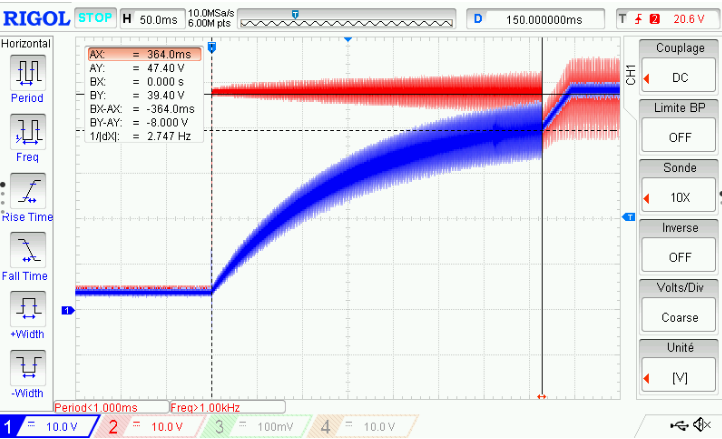
\includegraphics[width=0.75\linewidth]{assets/Chap3/Result_Freyche_Capa.png}
    \caption{Résultat de la mesure du condensateur du rapport de Thomas Freyche \cite{Freyche}}
    \label{fig:ResFreycheCapa}
\end{figure}

Lors de la mesure effectuée pour ce travail, un résultat identique a été obtenu, comme le montre la figure \ref{fig:ResCanCapa} :

\begin{figure}[H]
    \centering
    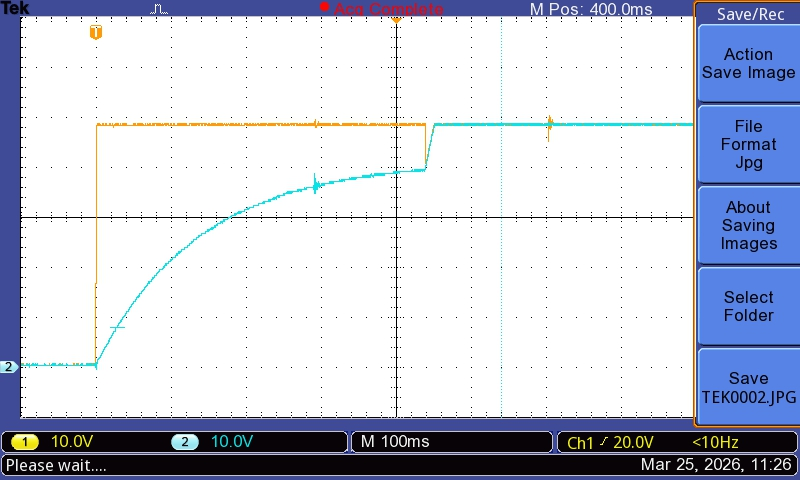
\includegraphics[width=0.75\linewidth]{assets/Chap3/MesureCondoCan.JPG}
    \caption{Résultat de la mesure du condensateur personnel}
    \label{fig:ResCanCapa}
\end{figure}

Cela vient prouver le bon fonctionnement du circuit de précharge.

\section{Mesure des régulateurs}

Cette section traite des mesures réalisées sur les régulateurs de la carte principale. Ces composants assurent l'alimentation correcte de l'intégralité du système.\\

Le convertisseur 24 V présente les résultats consignés dans le tableau \ref{tab:reg_24v_48v} :

\begin{table}[H]
    \centering
    \resizebox{\textwidth}{!}{%
        \begin{tabular}{|c|l|c|c|c|c|c|}
            \hline
            \multicolumn{7}{|c|}{\textbf{Régulateurs 24V et entrée 48V (PS1)}}                                                                                                                                                              \\ \hline
            N°  & \multicolumn{1}{c|}{Mesure}          & Point de mesure & \begin{tabular}[c]{@{}c@{}}Valeur théorique\\ {[}V{]}\end{tabular} & \begin{tabular}[c]{@{}c@{}}Valeur\\ mesurée {[}V{]}\end{tabular} & Erreur & Erreur {[}\%]{} \\ \hline
            1.a & Entrée des 48V                       & Bornie d'entrée & 48                                                                 & 48.05                                                            & 0.05   & 0.10            \\ \hline
            1.b & Tension après le switch de précharge & TP4             & 48                                                                 & 48.04                                                            & 0.04   & 0.08            \\ \hline
            2.a & Sortie du régulateur 24V             & TP6 et TP8      & 24                                                                 & 23.85                                                            & 0.15   & 0.62            \\ \hline
        \end{tabular}%
    }
    \caption{Mesures sur les régulateurs 24V et l'entrée 48V (PS1)}
    \label{tab:reg_24v_48v}
\end{table}

Le régulateur de 15 V présente les résultats consignés dans le tableau \ref{tab:reg_15v} :

\begin{table}[H]
    \centering
    \resizebox{\textwidth}{!}{%
        \begin{tabular}{|c|l|c|c|c|c|c|}
            \hline
            \multicolumn{7}{|c|}{\textbf{Régulateurs 15V (PS2)}}                                                                                                                                                                      \\ \hline
            N°  & \multicolumn{1}{c|}{Mesure} & Point de mesure    & \begin{tabular}[c]{@{}c@{}}Valeur théorique\\ {[}V{]}\end{tabular} & \begin{tabular}[c]{@{}c@{}}Valeur\\ mesurée {[}V{]}\end{tabular} & Erreur & Erreur {[}\%]{} \\ \hline
            1.a & Entrée des 24V              & Côté C12 de la C13 & 24                                                                 & 23.07                                                            & 0.93   & 3.88            \\ \hline
            2.a & Sortie du régulateur 15V    & TP1                & 15                                                                 & 14.95                                                            & 0.05   & 0.333           \\ \hline
        \end{tabular}%
    }
    \caption{Mesures sur le régulateur 15V (PS2)}
    \label{tab:reg_15v}
\end{table}

Le régulateur de 5 V présente les résultats consignés dans le tableau \ref{tab:reg_5v} :

\begin{table}[H]
    \centering
    \resizebox{\textwidth}{!}{%
        \begin{tabular}{|c|l|c|c|c|c|c|}
            \hline
            \multicolumn{7}{|c|}{\textbf{Régulateurs 5V (IC1)}}                                                                                                                                                                    \\ \hline
            N°  & \multicolumn{1}{c|}{Mesure} & Point de mesure & \begin{tabular}[c]{@{}c@{}}Valeur théorique\\ {[}V{]}\end{tabular} & \begin{tabular}[c]{@{}c@{}}Valeur\\ mesurée {[}V{]}\end{tabular} & Erreur & Erreur {[}\%]{} \\ \hline
            1.a & Entrée des 24V              & Pin 1 IC1       & 24                                                                 & 23.86                                                            & 0.14   & 0.583           \\ \hline
            2.a & Sortie du régulateur 5V     & L2 côté condo   & 5                                                                  & 4.989                                                            & 0.011  & 0.220           \\ \hline
            2.b & Après l'inducteur L2        & TP2             & 5                                                                  & 4.987                                                            & 0.013  & 0.260           \\ \hline
        \end{tabular}%
    }
    \caption{Mesures sur les régulateurs 5V (IC1)}
    \label{tab:reg_5v}
\end{table}

Le régulateur de 3,3 V présente les résultats consignés dans le tableau \ref{tab:reg_3_3v} :

\begin{table}[H]
    \centering
    \resizebox{\textwidth}{!}{%
        \begin{tabular}{|c|l|c|c|c|c|c|}
            \hline
            \multicolumn{7}{|c|}{\textbf{Régulateurs 3.3V (U6)}}                                                                                                                                                                   \\ \hline
            N°  & \multicolumn{1}{c|}{Mesure} & Point de mesure & \begin{tabular}[c]{@{}c@{}}Valeur théorique\\ {[}V{]}\end{tabular} & \begin{tabular}[c]{@{}c@{}}Valeur\\ mesurée {[}V{]}\end{tabular} & Erreur & Erreur {[}\%]{} \\ \hline
            1.a & Entrée des 5V               & J5 pin 2        & 5                                                                  & 4.982                                                            & 0.018  & 0.360           \\ \hline
            2.a & Sortie du régulateur 3.3V   & TP5             & 3.3                                                                & 3.296                                                            & 0.004  & 0.121           \\ \hline
        \end{tabular}%
    }
    \caption{Mesures sur les régulateurs 3.3V (U6)}
    \label{tab:reg_3_3v}
\end{table}

Le régulateur de 0,5 V présente les résultats consignés dans le tableau \ref{tab:reg_0_5v} :

\begin{table}[H]
    \centering
    \resizebox{\textwidth}{!}{%
        \begin{tabular}{|c|l|c|c|c|c|c|}
            \hline
            \multicolumn{7}{|c|}{\textbf{Régulateurs 0.5V (U5)}}                                                                                                                                                                   \\ \hline
            N°  & \multicolumn{1}{c|}{Mesure} & Point de mesure & \begin{tabular}[c]{@{}c@{}}Valeur théorique\\ {[}V{]}\end{tabular} & \begin{tabular}[c]{@{}c@{}}Valeur\\ mesurée {[}V{]}\end{tabular} & Erreur & Erreur {[}\%]{} \\ \hline
            1.a & Entrée des 24V              & C18 côté U6     & 5                                                                  & 4.981                                                            & 0.019  & 0.380           \\ \hline
            2.a & Sortie du régulateur 15V    & TP3             & 0.5                                                                & 0.4982                                                           & 0.002  & 0.360           \\ \hline
        \end{tabular}%
    }
    \caption{Mesures sur les régulateurs 0.5V (U5)}
    \label{tab:reg_0_5v}
\end{table}

\subsection{Analyse des résultats}
Les différents régulateurs présentés ci-dessus fonctionnent de manière nominale. Les tensions fournies sont conformes aux spécifications des constructeurs, ce qui garantit une alimentation stable pour l'ensemble de la carte.

Une anomalie a néanmoins été détectée sur le convertisseur 24 V lors des essais. Une broche mal soudée provoquait l'apparition d'arcs électriques sous le circuit imprimé. Ce module devra donc faire l'objet d'une attention particulière en cas de futurs dysfonctionnements électriques. Après la reprise de la soudure, le phénomène a été éliminé.

\section{Mesure des capteurs de courants}
\red{IL FAUT REFAIRE LES TABLEAUX. LA FORCE éTAIT MAL CALCULé DE PLUS çA MONTRE QUE LE COURANT CALCULé MONTRE QUE LA MASSE EST FAUSSE PUISQUE LA MAQUETTE A BESOIN DE CONSOMME PLUS DE COURANT. IL EST POSSIBLE DE CALCULER LA MASSE A PARTIR DU COURANT MESURé}
Cette section traite des différentes mesures réalisées afin de vérifier le comportement des capteurs de courant.

Dans un premier temps, une évaluation globale du bon fonctionnement des composants situés entre le capteur de courant et l'étage de réception des données par l'ADC a été effectuée.

Par la suite, le chariot a été soulevé uniquement du côté avant ou arrière. Cette manipulation permet de modifier la répartition de la force de pesanteur et d'alourdir localement la charge sur les inducteurs concernés. En fonctionnement nominal, la force électromécanique générée doit compenser cette charge pour maintenir la lévitation. La sustentation simultanée sur les quatre inducteurs n'étant pas exploitable au moment des tests, l'analyse s'est concentrée sur le soulèvement isolé de l'avant ou de l'arrière. L'application de ces charges connues offre la possibilité de calculer théoriquement le courant requis à partir de la force appliquée et des valeurs nominales de l'entrefer.

Cette série de mesures a été effectuée avant la découverte de la modification de la masse globale du système. Pour cette raison, le calcul du courant théorique s'appuie sur une masse de 3,4~kg par inducteur. Cette démarche permet de maintenir la cohérence avec le code source qui, au moment des essais, exploitait les coefficients ainsi que la commande a priori dimensionnés pour une masse totale de 13,6~kg.

\subsection{Mesure des circuits de conditionnement des capteurs de courants}

Les mesures globales des circuits de conditionnement sont présentées dans les tableaux \ref{tab:cond_courant_1} et \ref{tab:cond_courant_2} :


\begin{table}[H]
    \centering
    \resizebox{\textwidth}{!}{%
        \begin{tabular}{|c|c|c|c|c|c|c|}
            \hline
            \multicolumn{7}{|c|}{\textbf{Vérification général des conditionneurs de courant}}                                                                                                                                                                                                                                                             \\ \hline
            N°  & Mesure                                                                & \begin{tabular}[c]{@{}c@{}}Point de\\ mesure\end{tabular}   & \begin{tabular}[c]{@{}c@{}}Valeur théorique\\ {[}V{]}\end{tabular} & \begin{tabular}[c]{@{}c@{}}Valeur mesurée\\ {[}V{]}\end{tabular} & Erreur                                  & Erreur {[}\%{]} \\ \hline
            1.a & \begin{tabular}[c]{@{}c@{}}Alimentation de\\ l'AOP U1\_4\end{tabular} & U1\_4 pin 8                                                 & 5                                                                  & 4.989                                                            & 0.0110                                  & 0.2200          \\ \hline
            1.b & \begin{tabular}[c]{@{}c@{}}Alimentation de\\ l'AOP U2\_4\end{tabular} & U2\_4 pin 8                                                 & 3.3                                                                & 3.296                                                            & 0.0040                                  & 0.1212          \\ \hline
            1.c & \begin{tabular}[c]{@{}c@{}}Sortie du capteur\\ 1\end{tabular}         & \begin{tabular}[c]{@{}c@{}}R3\_4 côté\\ droite\end{tabular} & 0.625..4.375                                                       & 2.933                                                            & \multicolumn{2}{c|}{\multirow{3}{*}{-}}                   \\ \cline{1-5}
            1.d & \begin{tabular}[c]{@{}c@{}}Sortie de l'AOP\\ U1\_4\end{tabular}       & U2\_4 pin 5                                                 & 0.5..3.5                                                           & 1.173                                                            & \multicolumn{2}{c|}{}                                     \\ \cline{1-5}
            1.e & \begin{tabular}[c]{@{}c@{}}Sortie de l'AOP\\ U2\_4\end{tabular}       & TP9\_4                                                      & 0..3                                                               & 1.888                                                            & \multicolumn{2}{c|}{}                                     \\ \hline
            2.a & \begin{tabular}[c]{@{}c@{}}Alimentation de\\ l'AOP U1\_1\end{tabular} & U1\_1 pin 8                                                 & 5                                                                  & 4.984                                                            & 0.0160                                  & 0.3200          \\ \hline
            2.b & \begin{tabular}[c]{@{}c@{}}Alimentation de\\ l'AOP U2\_1\end{tabular} & U2\_1 pin 8                                                 & 3.3                                                                & 3.296                                                            & 0.0040                                  & 0.1212          \\ \hline
            2.c & \begin{tabular}[c]{@{}c@{}}Sortie du capteur\\ 2\end{tabular}         & \begin{tabular}[c]{@{}c@{}}R9\_1 côté\\ gauche\end{tabular} & 0.625..4.375                                                       & 2.872                                                            & \multicolumn{2}{c|}{\multirow{3}{*}{-}}                   \\ \cline{1-5}
            2.d & \begin{tabular}[c]{@{}c@{}}Sortie de l'AOP\\ U1\_1\end{tabular}       & U2\_1 pin 5                                                 & 0.5..3.5                                                           & 1.139                                                            & \multicolumn{2}{c|}{}                                     \\ \cline{1-5}
            2.e & \begin{tabular}[c]{@{}c@{}}Sortie de l'AOP\\ U2\_1\end{tabular}       & TP9\_1                                                      & 0..3                                                               & 1.736                                                            & \multicolumn{2}{c|}{}                                     \\ \hline
        \end{tabular}%
    }
    \caption{Vérification générale des conditionneurs de courant (Capteurs 1 et 2)}
    \label{tab:cond_courant_1}
\end{table}

\begin{table}[h!]
    \centering
    \resizebox{\textwidth}{!}{%
        \begin{tabular}{|c|c|c|c|c|c|c|}
            \hline
            \multicolumn{7}{|c|}{\textbf{Vérification général des conditionneurs de courant}}                                                                                                                                                                                                                                                             \\ \hline
            N°  & Mesure                                                                & \begin{tabular}[c]{@{}c@{}}Point de\\ mesure\end{tabular}   & \begin{tabular}[c]{@{}c@{}}Valeur théorique\\ {[}V{]}\end{tabular} & \begin{tabular}[c]{@{}c@{}}Valeur mesurée\\ {[}V{]}\end{tabular} & Erreur                                  & Erreur {[}\%{]} \\ \hline
            3.a & \begin{tabular}[c]{@{}c@{}}Alimentation de\\ l'AOP U1\_3\end{tabular} & U1\_3 pin 8                                                 & 5                                                                  & 4.985                                                            & 0.0150                                  & 0.3000          \\ \hline
            3.b & \begin{tabular}[c]{@{}c@{}}Alimentation de\\ l'AOP U2\_3\end{tabular} & U2\_3 pin 8                                                 & 3.3                                                                & 3.296                                                            & 0.0040                                  & 0.1212          \\ \hline
            3.c & \begin{tabular}[c]{@{}c@{}}Sortie du capteur\\ 3\end{tabular}         & \begin{tabular}[c]{@{}c@{}}R9\_3 côté\\ droite\end{tabular} & 0.625..4.375                                                       & 2.485                                                            & \multicolumn{2}{c|}{\multirow{3}{*}{-}}                   \\ \cline{1-5}
            3.d & \begin{tabular}[c]{@{}c@{}}Sortie de l'AOP\\ U1\_3\end{tabular}       & U2\_3 pin 5                                                 & 0.5..3.5                                                           & 0.996                                                            & \multicolumn{2}{c|}{}                                     \\ \cline{1-5}
            3.e & \begin{tabular}[c]{@{}c@{}}Sortie de l'AOP\\ U2\_3\end{tabular}       & TP9\_3                                                      & 0..3                                                               & 1.532                                                            & \multicolumn{2}{c|}{}                                     \\ \hline
            4.a & \begin{tabular}[c]{@{}c@{}}Alimentation de\\ l'AOP U1\_2\end{tabular} & U1\_2 pin 8                                                 & 5                                                                  & 4.984                                                            & 0.0160                                  & 0.3200          \\ \hline
            4.b & \begin{tabular}[c]{@{}c@{}}Alimentation de\\ l'AOP U2\_2\end{tabular} & U2\_2 pin 8                                                 & 3.300                                                              & 3.296                                                            & 0.0040                                  & 0.1212          \\ \hline
            4.c & \begin{tabular}[c]{@{}c@{}}Sortie du capteur\\ 4\end{tabular}         & \begin{tabular}[c]{@{}c@{}}R9\_2 côté\\ gauche\end{tabular} & 0.625..4.375                                                       & 2.498                                                            & \multicolumn{2}{c|}{\multirow{3}{*}{-}}                   \\ \cline{1-5}
            4.d & \begin{tabular}[c]{@{}c@{}}Sortie de l'AOP\\ U1\_2\end{tabular}       & U2\_2 pin 5                                                 & 0.5..3.5                                                           & 0.999                                                            & \multicolumn{2}{c|}{}                                     \\ \cline{1-5}
            4.e & \begin{tabular}[c]{@{}c@{}}Sortie de l'AOP\\ U2\_2\end{tabular}       & TP9\_2                                                      & 0..3                                                               & 1.545                                                            & \multicolumn{2}{c|}{}                                     \\ \hline
        \end{tabular}%
    }
    \caption{Vérification générale des conditionneurs de courant (Capteurs 3 et 4)}
    \label{tab:cond_courant_2}
\end{table}

\subsection{Mesure du courant sans ajout de poids}
Une première série de mesures a été réalisée sans ajout de masse afin d'établir des comparaisons entre les valeurs théoriques, les mesures par sonde de courant et les données acquises par l'ADC. Ces résultats sont consignés dans les tableaux \ref{tab:sans_poids_sonde}, \ref{tab:sans_poids_adc} et \ref{tab:sans_poids_comp} :

% --- Sans Poids - Partie 1 (Sonde) ---
\begin{table}[H]
    \centering
    \resizebox{\textwidth}{!}{%
        \begin{tabular}{|c|c|c|c|c|c|c|c|c|c|}
            \hline
            \multicolumn{10}{|c|}{\textbf{Sans poids}}                                                                                                                                                                                                                                                                                                                                                                                                                                                               \\ \hline
            Inducteur & \begin{tabular}[c]{@{}c@{}}Position\\ {[}m{]}\end{tabular} & L {[}H{]}                 & \begin{tabular}[c]{@{}c@{}}k\\ {[}m*A/N{]}\end{tabular} & \begin{tabular}[c]{@{}c@{}}Masse\\ {[}kg{]}\end{tabular} & \begin{tabular}[c]{@{}c@{}}Force\\ {[}N{]}\end{tabular} & \begin{tabular}[c]{@{}c@{}}Courant\\ théorique {[}A{]}\end{tabular} & \begin{tabular}[c]{@{}c@{}}Courant\\ mesuré {[}A{]}\end{tabular} & Erreur & \begin{tabular}[c]{@{}c@{}}Erreur\\ relative {[}\%{]}\end{tabular} \\ \hline
            1         & \multirow{4}{*}{2.00E-03}                                  & \multirow{4}{*}{4.90E-03} & \multirow{4}{*}{4.90E-06}                               & \multirow{4}{*}{6.8}                                     & 67                                                      & 7.4                                                                 & 6.1                                                              & 1.3    & 18                                                                 \\ \cline{1-1} \cline{6-10}
            2         &                                                            &                           &                                                         &                                                          & 67                                                      & 7.4                                                                 & 6.2                                                              & 1.2    & 17                                                                 \\ \cline{1-1} \cline{6-10}
            3         &                                                            &                           &                                                         &                                                          & 67                                                      & 7.4                                                                 & 6.4                                                              & 1.0    & 13                                                                 \\ \cline{1-1} \cline{6-10}
            4         &                                                            &                           &                                                         &                                                          & 67                                                      & 7.4                                                                 & 5.8                                                              & 1.5    & 21                                                                 \\ \hline
        \end{tabular}%
    }
    \caption{Mesures de courant par sonde (Sans poids, 6.8 kg)}
    \label{tab:sans_poids_sonde}
\end{table}

% --- Sans Poids - Partie 2 (ADC) ---
\begin{table}[H]
    \centering
    \resizebox{\textwidth}{!}{%
        \begin{tabular}{|c|c|c|c|c|c|c|c|c|c|}
            \hline
            \multicolumn{10}{|c|}{\textbf{Sans poids}}                                                                                                                                                                                                                                                                                                                                                                                                                                                    \\ \hline
            Inducteur & \begin{tabular}[c]{@{}c@{}}Position\\ {[}m{]}\end{tabular} & L {[}H{]}                 & \begin{tabular}[c]{@{}c@{}}k\\ {[}m*A/N{]}\end{tabular} & \begin{tabular}[c]{@{}c@{}}Masse\\ {[}kg{]}\end{tabular} & \begin{tabular}[c]{@{}c@{}}Force\\ {[}N{]}\end{tabular} & \begin{tabular}[c]{@{}c@{}}Courant\\ théorique {[}A{]}\end{tabular} & \begin{tabular}[c]{@{}c@{}}ADC\\ {[}A{]}\end{tabular} & Erreur & \begin{tabular}[c]{@{}c@{}}Erreur\\ relative {[}\%{]}\end{tabular} \\ \hline
            1         & \multirow{4}{*}{2.00E-03}                                  & \multirow{4}{*}{4.90E-03} & \multirow{4}{*}{4.90E-06}                               & \multirow{4}{*}{6.8}                                     & 66.7                                                    & 7.38                                                                & 6.79                                                  & 0.594  & 8.05                                                               \\ \cline{1-1} \cline{6-10}
            2         &                                                            &                           &                                                         &                                                          & 66.7                                                    & 7.38                                                                & 6.45                                                  & 0.933  & 12.6                                                               \\ \cline{1-1} \cline{6-10}
            3         &                                                            &                           &                                                         &                                                          & 66.7                                                    & 7.38                                                                & 6.54                                                  & 0.841  & 11.4                                                               \\ \cline{1-1} \cline{6-10}
            4         &                                                            &                           &                                                         &                                                          & 66.7                                                    & 7.38                                                                & 6.02                                                  & 1.36   & 18.5                                                               \\ \hline
        \end{tabular}%
    }
    \caption{Mesures de courant par ADC (Sans poids, 6.8 kg)}
    \label{tab:sans_poids_adc}
\end{table}

% --- Sans Poids - Partie 3 (Comparatif) ---
\begin{table}[H]
    \centering
    \begin{tabular}{|c|c|c|c|}
        \hline
        \multicolumn{4}{|c|}{\textbf{Sans poids}}        \\ \hline
        Inducteur & ADC {[}A{]} & Sonde {[}A{]} & Erreur \\ \hline
        1         & 6.79        & 6.08          & 0.71   \\ \hline
        2         & 6.45        & 6.16          & 0.29   \\ \hline
        3         & 6.54        & 6.40          & 0.14   \\ \hline
        4         & 6.02        & 5.84          & 0.18   \\ \hline
    \end{tabular}
    \caption{Comparatif des erreurs entre l'ADC et la sonde (Sans poids, 6.8 kg)}
    \label{tab:sans_poids_comp}
\end{table}

\subsection{Mesure du courant avec une masse de 1.25kg}
Selon le même principe, des essais ont été effectués en ajoutant une masse d'environ 1,25 kg. Afin de garantir une précision maximale, ces masses ont été pesées au préalable pour obtenir une valeur de charge exacte. Les mesures correspondantes sont présentées dans les tableaux \ref{tab:poids_1_25_sonde}, \ref{tab:poids_1_25_adc} et \ref{tab:poids_1_25_comp} :

% --- Poids 1.25 kg - Partie 1 (Sonde) ---
\begin{table}[H]
    \centering
    \resizebox{\textwidth}{!}{%
        \begin{tabular}{|c|c|c|c|c|c|c|c|c|c|}
            \hline
            \multicolumn{10}{|c|}{\textbf{Poids de 1.25 kg}}                                                                                                                                                                                                                                                                                                                                                                                                                                                         \\ \hline
            Inducteur & \begin{tabular}[c]{@{}c@{}}Position\\ {[}m{]}\end{tabular} & L {[}H{]}                 & \begin{tabular}[c]{@{}c@{}}k\\ {[}m*A/N{]}\end{tabular} & \begin{tabular}[c]{@{}c@{}}Masse\\ {[}kg{]}\end{tabular} & \begin{tabular}[c]{@{}c@{}}Force\\ {[}N{]}\end{tabular} & \begin{tabular}[c]{@{}c@{}}Courant\\ théorique {[}A{]}\end{tabular} & \begin{tabular}[c]{@{}c@{}}Courant\\ mesuré {[}A{]}\end{tabular} & Erreur & \begin{tabular}[c]{@{}c@{}}Erreur\\ relative {[}\%{]}\end{tabular} \\ \hline
            1         & \multirow{4}{*}{2.00E-03}                                  & \multirow{4}{*}{4.90E-03} & \multirow{4}{*}{4.90E-06}                               & 8.0                                                      & 78.7                                                    & 8.02                                                                & 7.6                                                              & 0.4    & 5.2                                                                \\ \cline{1-1} \cline{5-10}
            2         &                                                            &                           &                                                         & 8.0                                                      & 78.5                                                    & 8.00                                                                & 7.2                                                              & 0.8    & 10                                                                 \\ \cline{1-1} \cline{5-10}
            3         &                                                            &                           &                                                         & 8.0                                                      & 78.7                                                    & 8.02                                                                & 7.4                                                              & 0.6    & 7.7                                                                \\ \cline{1-1} \cline{5-10}
            4         &                                                            &                           &                                                         & 8.0                                                      & 78.5                                                    & 8.00                                                                & 7.2                                                              & 0.8    & 10                                                                 \\ \hline
        \end{tabular}%
    }
    \caption{Mesures de courant par sonde (Poids de 1.25 kg, 8.0 kg)}
    \label{tab:poids_1_25_sonde}
\end{table}

% --- Poids 1.25 kg - Partie 2 (ADC) ---
\begin{table}[H]
    \centering
    \resizebox{\textwidth}{!}{%
        \begin{tabular}{|c|c|c|c|c|c|c|c|c|c|}
            \hline
            \multicolumn{10}{|c|}{\textbf{Poids de 1.25 kg}}                                                                                                                                                                                                                                                                                                                                                                                                                                              \\ \hline
            Inducteur & \begin{tabular}[c]{@{}c@{}}Position\\ {[}m{]}\end{tabular} & L {[}H{]}                 & \begin{tabular}[c]{@{}c@{}}k\\ {[}m*A/N{]}\end{tabular} & \begin{tabular}[c]{@{}c@{}}Masse\\ {[}kg{]}\end{tabular} & \begin{tabular}[c]{@{}c@{}}Force\\ {[}N{]}\end{tabular} & \begin{tabular}[c]{@{}c@{}}Courant\\ théorique {[}A{]}\end{tabular} & \begin{tabular}[c]{@{}c@{}}ADC\\ {[}A{]}\end{tabular} & Erreur & \begin{tabular}[c]{@{}c@{}}Erreur\\ relative {[}\%{]}\end{tabular} \\ \hline
            1         & \multirow{4}{*}{2.00E-03}                                  & \multirow{4}{*}{4.90E-03} & \multirow{4}{*}{4.90E-06}                               & 8.0                                                      & 78.7                                                    & 8.02                                                                & 7.98                                                  & 0.039  & 0.491                                                              \\ \cline{1-1} \cline{5-10}
            2         &                                                            &                           &                                                         & 8.0                                                      & 78.5                                                    & 8.00                                                                & 7.26                                                  & 0.743  & 9.28                                                               \\ \cline{1-1} \cline{5-10}
            3         &                                                            &                           &                                                         & 8.0                                                      & 78.7                                                    & 8.02                                                                & 7.47                                                  & 0.552  & 6.89                                                               \\ \cline{1-1} \cline{5-10}
            4         &                                                            &                           &                                                         & 8.0                                                      & 78.5                                                    & 8.00                                                                & 7.10                                                  & 0.906  & 11.3                                                               \\ \hline
        \end{tabular}%
    }
    \caption{Mesures de courant par ADC (Poids de 1.25 kg, 8.0 kg)}
    \label{tab:poids_1_25_adc}
\end{table}

% --- Poids 1.25 kg - Partie 3 (Comparatif) ---
\begin{table}[H]
    \centering
    \begin{tabular}{|c|c|c|c|}
        \hline
        \multicolumn{4}{|c|}{\textbf{Poids de 1.25 kg}}  \\ \hline
        Inducteur & ADC {[}A{]} & Sonde {[}A{]} & Erreur \\ \hline
        1         & 8.0         & 7.6           & 0.38   \\ \hline
        2         & 7.3         & 7.2           & 0.060  \\ \hline
        3         & 7.5         & 7.4           & 0.065  \\ \hline
        4         & 7.1         & 7.2           & 0.10   \\ \hline
    \end{tabular}
    \caption{Comparatif des erreurs entre l'ADC et la sonde (Poids de 1.25 kg, 8.0 kg)}
    \label{tab:poids_1_25_comp}
\end{table}

\subsection{Mesure du courant avec une masse de 2.5kg}
Enfin, une charge d'environ 2,5~kg a été ajoutée pour clore les essais. Les résultats de ces mesures sont détaillés dans les tableaux \ref{tab:poids_2_5_sonde}, \ref{tab:poids_2_5_adc} et \ref{tab:poids_2_5_comp} :

% --- Poids 2.5 kg - Partie 1 (Sonde) ---
\begin{table}[H]
    \centering
    \resizebox{\textwidth}{!}{%
        \begin{tabular}{|c|c|c|c|c|c|c|c|c|c|}
            \hline
            \multicolumn{10}{|c|}{\textbf{Poids de 2.5 kg}}                                                                                                                                                                                                                                                                                                                                                                                                                                                          \\ \hline
            Inducteur & \begin{tabular}[c]{@{}c@{}}Position\\ {[}m{]}\end{tabular} & L {[}H{]}                 & \begin{tabular}[c]{@{}c@{}}k\\ {[}m*A/N{]}\end{tabular} & \begin{tabular}[c]{@{}c@{}}Masse\\ {[}kg{]}\end{tabular} & \begin{tabular}[c]{@{}c@{}}Force\\ {[}N{]}\end{tabular} & \begin{tabular}[c]{@{}c@{}}Courant\\ théorique {[}A{]}\end{tabular} & \begin{tabular}[c]{@{}c@{}}Courant\\ mesuré {[}A{]}\end{tabular} & Erreur & \begin{tabular}[c]{@{}c@{}}Erreur\\ relative {[}\%{]}\end{tabular} \\ \hline
            1         & \multirow{4}{*}{2.00E-03}                                  & \multirow{4}{*}{4.90E-03} & \multirow{4}{*}{4.90E-06}                               & 9.2                                                      & 91                                                      & 8.6                                                                 & 8.2                                                              & 0.40   & 4.6                                                                \\ \cline{1-1} \cline{5-10}
            2         &                                                            &                           &                                                         & 9.3                                                      & 91                                                      & 8.6                                                                 & 8.2                                                              & 0.42   & 4.8                                                                \\ \cline{1-1} \cline{5-10}
            3         &                                                            &                           &                                                         & 9.2                                                      & 91                                                      & 8.6                                                                 & 8.2                                                              & 0.40   & 4.6                                                                \\ \cline{1-1} \cline{5-10}
            4         &                                                            &                           &                                                         & 9.3                                                      & 91                                                      & 8.6                                                                 & 8.8                                                              & 0.18   & 2.1                                                                \\ \hline
        \end{tabular}%
    }
    \caption{Mesures de courant par sonde (Poids de 2.5 kg, 9.2 kg)}
    \label{tab:poids_2_5_sonde}
\end{table}

% --- Poids 2.5 kg - Partie 2 (ADC) ---
\begin{table}[H]
    \centering
    \resizebox{\textwidth}{!}{%
        \begin{tabular}{|c|c|c|c|c|c|c|c|c|c|}
            \hline
            \multicolumn{10}{|c|}{\textbf{Poids de 2.5 kg}}                                                                                                                                                                                                                                                                                                                                                                                                                                               \\ \hline
            Inducteur & \begin{tabular}[c]{@{}c@{}}Position\\ {[}m{]}\end{tabular} & L {[}H{]}                 & \begin{tabular}[c]{@{}c@{}}k\\ {[}m*A/N{]}\end{tabular} & \begin{tabular}[c]{@{}c@{}}Masse\\ {[}kg{]}\end{tabular} & \begin{tabular}[c]{@{}c@{}}Force\\ {[}N{]}\end{tabular} & \begin{tabular}[c]{@{}c@{}}Courant\\ théorique {[}A{]}\end{tabular} & \begin{tabular}[c]{@{}c@{}}ADC\\ {[}A{]}\end{tabular} & Erreur & \begin{tabular}[c]{@{}c@{}}Erreur\\ relative {[}\%{]}\end{tabular} \\ \hline
            1         & \multirow{4}{*}{2.00E-03}                                  & \multirow{4}{*}{4.90E-03} & \multirow{4}{*}{4.90E-06}                               & 9.2                                                      & 90.6                                                    & 8.60                                                                & 8.93                                                  & 0.325  & 3.78                                                               \\ \cline{1-1} \cline{5-10}
            2         &                                                            &                           &                                                         & 9.3                                                      & 90.9                                                    & 8.62                                                                & 8.29                                                  & 0.323  & 3.75                                                               \\ \cline{1-1} \cline{5-10}
            3         &                                                            &                           &                                                         & 9.2                                                      & 90.6                                                    & 8.60                                                                & 8.05                                                  & 0.548  & 6.37                                                               \\ \cline{1-1} \cline{5-10}
            4         &                                                            &                           &                                                         & 9.3                                                      & 90.9                                                    & 8.62                                                                & 8.78                                                  & 0.162  & 1.88                                                               \\ \hline
        \end{tabular}%
    }
    \caption{Mesures de courant par ADC (Poids de 2.5 kg, 9.2 kg)}
    \label{tab:poids_2_5_adc}
\end{table}

% --- Poids 2.5 kg - Partie 3 (Comparatif) ---
\begin{table}[H]
    \centering
    \begin{tabular}{|c|c|c|c|}
        \hline
        \multicolumn{4}{|c|}{\textbf{Poids de 2.5 kg}}   \\ \hline
        Inducteur & ADC {[}A{]} & Sonde {[}A{]} & Erreur \\ \hline
        1         & 8.9         & 8.2           & 0.73   \\ \hline
        2         & 8.3         & 8.2           & 0.093  \\ \hline
        3         & 8.1         & 8.2           & 0.15   \\ \hline
        4         & 8.8         & 8.8           & 0.022  \\ \hline
    \end{tabular}
    \caption{Comparatif des erreurs entre l'ADC et la sonde (Poids de 2.5 kg, 9.2 kg)}
    \label{tab:poids_2_5_comp}
\end{table}

\subsection{Analyse des résultats}
Comme le montrent les tableaux \ref{tab:sans_poids_sonde}, \ref{tab:sans_poids_adc}, \ref{tab:poids_1_25_sonde}, \ref{tab:poids_1_25_adc}, \ref{tab:poids_2_5_sonde} et \ref{tab:poids_2_5_adc}, les valeurs mesurées (via la sonde ou l'ADC) convergent vers les valeurs théoriques, bien qu'un certain écart subsiste. Cet écart engendre des erreurs relatives non négligeables. Ce phénomène s'explique par le fait que seule une extrémité du chariot (l'avant ou l'arrière) était soulevée lors des essais ; le point d'appui resté en contact avec le sol agit indirectement comme un support mécanique, modifiant ainsi la charge réelle supportée individuellement par chaque inducteur.

En comparant les deux méthodes de mesure à travers les tableaux \ref{tab:sans_poids_comp}, \ref{tab:poids_1_25_comp} et \ref{tab:poids_2_5_comp}, une forte similarité entre les résultats est observée. Cela démontre que l'acquisition de données est correcte et qu'il y a une bonne correspondance entre le courant circulant réellement dans l'inducteur et la valeur mesurée par le capteur.

Le fonctionnement du capteur de courant est donc validé et considéré comme correct.

\section{Mesure des capteurs de position}
Cette section traite des mesures réalisées sur les capteurs de position. De nombreuses séries d'essais ont été effectuées afin de tester différents étalonnages. Par conséquent, seules les approches les plus pertinentes ont été conservées afin d'alléger le contenu de ce document.

Les mesures ont été réalisées à l'aide de cales de différentes épaisseurs (1~mm, 1,5~mm, 2~mm et 3~mm). Ces éléments permettaient de surélever la partie mobile et, ainsi, de réduire l'entrefer des bobines. Dans les relevés, un entrefer de 3~mm correspond à la position de repos théorique du chariot. Lorsqu'une cale de 2,5~mm est mentionnée, cela correspond à la superposition d'une cale de 1~mm et d'une cale de 1,5~mm.

\subsection{Mesure des circuits de conditionnement}
Dans un premier temps, une vérification globale des circuits de conditionnement a été effectuée, de manière analogue à la procédure suivie pour les capteurs de courant. Les résultats sont présentés dans le tableau \ref{tab:cond_position} :

\begin{table}[H]
    \centering
    \resizebox{\textwidth}{!}{%
        \begin{tabular}{|c|c|c|c|c|c|c|}
            \hline
            \multicolumn{7}{|c|}{\textbf{Vérification générale des conditionneurs de position}}                                                                                                                                                                                                                                                           \\ \hline
            N°  & Mesure                                                                & \begin{tabular}[c]{@{}c@{}}Point de\\ mesure\end{tabular}   & \begin{tabular}[c]{@{}c@{}}Valeur\\ théorique {[}V{]}\end{tabular} & \begin{tabular}[c]{@{}c@{}}Valeur\\ mesurée {[}V{]}\end{tabular} & Erreur                                  & Erreur {[}\%{]} \\ \hline
            1.a & \begin{tabular}[c]{@{}c@{}}Alimentation de\\ l'AOP U3\_4\end{tabular} & U3\_4 pin 8                                                 & 3.3                                                                & 3.30                                                             & 4E-03                                   & 0.12            \\ \hline
            1.c & Sortie du capteur 1                                                   & \begin{tabular}[c]{@{}c@{}}Connector 1\\ pin 2\end{tabular} & 0..10                                                              & 9.56                                                             & \multicolumn{2}{c|}{\multirow{2}{*}{-}}                   \\ \cline{1-5}
            1.d & Sortie de l'AOP U1\_4                                                 & TP12\_4                                                     & 0..3                                                               & 2.85                                                             & \multicolumn{2}{c|}{}                                     \\ \hline
            2.a & \begin{tabular}[c]{@{}c@{}}Alimentation de\\ l'AOP U3\_1\end{tabular} & U3\_1 pin 8                                                 & 3.3                                                                & 3.30                                                             & 4E-03                                   & 0.12            \\ \hline
            2.c & Sortie du capteur 2                                                   & \begin{tabular}[c]{@{}c@{}}Connector 2\\ pin 2\end{tabular} & 0..10                                                              & 9.74                                                             & \multicolumn{2}{c|}{\multirow{2}{*}{-}}                   \\ \cline{1-5}
            2.d & Sortie de l'AOP U3\_1                                                 & TP12\_1                                                     & 0..3                                                               & 2.91                                                             & \multicolumn{2}{c|}{}                                     \\ \hline
            3.a & \begin{tabular}[c]{@{}c@{}}Alimentation de\\ l'AOP U3\_3\end{tabular} & U3\_3 pin 8                                                 & 3.3                                                                & 3.30                                                             & 4E-03                                   & 0.12            \\ \hline
            3.c & Sortie du capteur 3                                                   & \begin{tabular}[c]{@{}c@{}}Connector 3\\ pin 2\end{tabular} & 0..10                                                              & 9.92                                                             & \multicolumn{2}{c|}{\multirow{2}{*}{-}}                   \\ \cline{1-5}
            3.d & Sortie de l'AOP U1\_3                                                 & U3\_3 pin 5                                                 & 0..3                                                               & 2.96                                                             & \multicolumn{2}{c|}{}                                     \\ \hline
            4.a & \begin{tabular}[c]{@{}c@{}}Alimentation de\\ l'AOP U3\_2\end{tabular} & U3\_2 pin 8                                                 & 3.3                                                                & 3.30                                                             & 4E-03                                   & 0.12            \\ \hline
            4.c & Sortie du capteur 4                                                   & \begin{tabular}[c]{@{}c@{}}Connector 4\\ pin 2\end{tabular} & 0..10                                                              & 10.0                                                             & \multicolumn{2}{c|}{\multirow{2}{*}{-}}                   \\ \cline{1-5}
            4.d & Sortie de l'AOP U3\_2                                                 & TP12\_2                                                     & 0..3                                                               & 2.99                                                             & \multicolumn{2}{c|}{}                                     \\ \hline
        \end{tabular}%
    }
    \caption{Vérification générale des conditionneurs de position}
    \label{tab:cond_position}
\end{table}

\subsection{Première mesure des capteurs de position}
La première série d'essais correspond à la configuration matérielle issue du précédent travail de bachelor. Les résultats obtenus sont détaillés dans les tableaux \ref{tab:premier_mesure_pos_cond} et \ref{tab:premier_mesure_pos_adc} :

% --- Tableau 1 : Après le conditionnement ---
\begin{table}[H]
    \centering
    \begin{tabular}{|c|c|c|c|c|}
        \hline
        \multicolumn{5}{|c|}{\textbf{Mesure des positions après le conditionnement}}                 \\ \hline
        Inducteur          & Théorique {[}V{]} & Mesurée {[}V{]} & Erreur & Erreur relative {[}\%{]} \\ \hline
        \multirow{3}{*}{1} & 1.000             & 1.043           & 0.043  & 4.300                    \\ \cline{2-5}
                           & 2.000             & 1.982           & 0.018  & 0.900                    \\ \cline{2-5}
                           & 3.000             & 2.986           & 0.014  & 0.467                    \\ \hline
        \multirow{3}{*}{2} & 1.000             & 0.994           & 0.006  & 0.600                    \\ \cline{2-5}
                           & 2.000             & 1.939           & 0.061  & 3.050                    \\ \cline{2-5}
                           & 3.000             & 2.962           & 0.038  & 1.267                    \\ \hline
        \multirow{3}{*}{3} & 1.000             & 0.763           & 0.237  & 23.700                   \\ \cline{2-5}
                           & 2.000             & 1.769           & 0.231  & 11.550                   \\ \cline{2-5}
                           & 3.000             & 2.891           & 0.109  & 3.633                    \\ \hline
        \multirow{3}{*}{4} & 1.000             & 0.942           & 0.058  & 5.800                    \\ \cline{2-5}
                           & 2.000             & 1.913           & 0.087  & 4.350                    \\ \cline{2-5}
                           & 3.000             & 2.970           & 0.030  & 1.000                    \\ \hline
    \end{tabular}
    \caption{Première mesure des tensions en sortie de la carte de conditionnement}
    \label{tab:premier_mesure_pos_cond}
\end{table}

% --- Tableau 2 : Après l'ADC ---
\begin{table}[H]
    \centering
    \begin{tabular}{|c|c|c|c|c|}
        \hline
        \multicolumn{5}{|c|}{\textbf{Mesure des positions après l'ADC}}                                \\ \hline
        Inducteur          & Théorique {[}mm{]} & Mesurée {[}mm{]} & Erreur & Erreur relative {[}\%{]} \\ \hline
        \multirow{3}{*}{1} & 1.000              & 1.050            & 0.050  & 5.000                    \\ \cline{2-5}
                           & 2.000              & 1.989            & 0.011  & 0.550                    \\ \cline{2-5}
                           & 3.000              & 3.006            & 0.006  & 0.200                    \\ \hline
        \multirow{3}{*}{2} & 1.000              & 1.005            & 0.005  & 0.500                    \\ \cline{2-5}
                           & 2.000              & 1.945            & 0.055  & 2.750                    \\ \cline{2-5}
                           & 3.000              & 2.970            & 0.030  & 1.000                    \\ \hline
        \multirow{3}{*}{3} & 1.000              & 0.790            & 0.210  & 21.000                   \\ \cline{2-5}
                           & 2.000              & 1.786            & 0.214  & 10.700                   \\ \cline{2-5}
                           & 3.000              & 2.897            & 0.103  & 3.433                    \\ \hline
        \multirow{3}{*}{4} & 1.000              & 0.939            & 0.061  & 6.100                    \\ \cline{2-5}
                           & 2.000              & 1.907            & 0.093  & 4.650                    \\ \cline{2-5}
                           & 3.000              & 2.968            & 0.032  & 1.067                    \\ \hline
    \end{tabular}
    \caption{Première mesure des positions en sortie de l'ADC}
    \label{tab:premier_mesure_pos_adc}
\end{table}

\subsection{Mesure après la calibration du capteur 3}
À la suite de ces résultats, une première calibration par la méthode d'apprentissage "Teach-In" a été effectuée sur le capteur de l'inducteur 3. Une série de mesures, de la sortie du capteur jusqu'à l'ADC, a été réalisée afin d'analyser l'évolution de la tension. Les relevés sont présentés dans les tableaux \ref{tab:teachin_3_capteurs}, \ref{tab:teachin_3_cond} et \ref{tab:teachin_3_adc} :

% --- Tableau 1 : Après la sortie des capteurs (Droite sur l'image) ---
\begin{table}[H]
    \centering
    \begin{tabular}{|c|c|c|c|c|}
        \hline
        \multicolumn{5}{|c|}{\textbf{Mesure des positions après la sortie des capteurs}}             \\ \hline
        Inducteur          & Théorique {[}V{]} & Mesurée {[}V{]} & Erreur & Erreur relative {[}\%{]} \\ \hline
        \multirow{4}{*}{1} & 0.00              & 0.711           & 0.711  & -                        \\ \cline{2-5}
                           & 3.33              & 2.95            & 0.383  & 11.5                     \\ \cline{2-5}
                           & 6.67              & 6.2             & 0.467  & 7                        \\ \cline{2-5}
                           & 10.0              & 9.63            & 0.370  & 3.7                      \\ \hline
        \multirow{4}{*}{2} & 0.00              & 0.2034          & 0.203  & -                        \\ \cline{2-5}
                           & 3.33              & 2.687           & 0.646  & 19.39                    \\ \cline{2-5}
                           & 6.67              & 6.04            & 0.627  & 9.4                      \\ \cline{2-5}
                           & 10.0              & 9.67            & 0.330  & 3.3                      \\ \hline
        \multirow{4}{*}{3} & 0.00              & 0.2255          & 0.226  & -                        \\ \cline{2-5}
                           & 3.33              & 2.437           & 0.896  & 26.89                    \\ \cline{2-5}
                           & 6.67              & 6.02            & 0.647  & 9.7                      \\ \cline{2-5}
                           & 10.00             & 9.87            & 0.130  & 1.3                      \\ \hline
        \multirow{4}{*}{4} & 0.00              & 0.2176          & 0.218  & -                        \\ \cline{2-5}
                           & 3.33              & 2.84            & 0.493  & 14.8                     \\ \cline{2-5}
                           & 6.67              & 6.11            & 0.557  & 8.35                     \\ \cline{2-5}
                           & 10.0              & 9.87            & 0.130  & 1.3                      \\ \hline
    \end{tabular}
    \caption{Mesure des tensions en sortie des capteurs (Calibration teach-in de l'inducteur 3)}
    \label{tab:teachin_3_capteurs}
\end{table}

% --- Tableau 2 : Après le conditionneur (Milieu sur l'image) ---
\begin{table}[H]
    \centering
    \begin{tabular}{|c|c|c|c|c|}
        \hline
        \multicolumn{5}{|c|}{\textbf{Mesure des positions après le conditionneur}}                   \\ \hline
        Inducteur          & Théorique {[}V{]} & Mesurée {[}V{]} & Erreur & Erreur relative {[}\%{]} \\ \hline
        \multirow{4}{*}{1} & 0                 & 0.189           & 0.189  & -                        \\ \cline{2-5}
                           & 1                 & 0.867           & 0.133  & 13.3                     \\ \cline{2-5}
                           & 2                 & 1.88            & 0.125  & 6.25                     \\ \cline{2-5}
                           & 3                 & 2.86            & 0.138  & 4.60                     \\ \hline
        \multirow{4}{*}{2} & 0                 & 0.100           & 0.100  & -                        \\ \cline{2-5}
                           & 1                 & 0.816           & 0.184  & 18.4                     \\ \cline{2-5}
                           & 2                 & 1.84            & 0.161  & 8.05                     \\ \cline{2-5}
                           & 3                 & 2.88            & 0.119  & 3.97                     \\ \hline
        \multirow{4}{*}{3} & 0                 & 0.040           & 0.040  & -                        \\ \cline{2-5}
                           & 1                 & 0.715           & 0.285  & 28.5                     \\ \cline{2-5}
                           & 2                 & 1.82            & 0.177  & 8.85                     \\ \cline{2-5}
                           & 3                 & 2.94            & 0.059  & 1.97                     \\ \hline
        \multirow{4}{*}{4} & 0                 & 0.070           & 0.070  & -                        \\ \cline{2-5}
                           & 1                 & 0.846           & 0.154  & 15.4                     \\ \cline{2-5}
                           & 2                 & 1.86            & 0.140  & 7                        \\ \cline{2-5}
                           & 3                 & 2.94            & 0.059  & 1.97                     \\ \hline
    \end{tabular}
    \caption{Mesure des tensions en sortie du conditionneur (Calibration teach-in de l'inducteur 3)}
    \label{tab:teachin_3_cond}
\end{table}

% --- Tableau 3 : Après l'ADC (Gauche sur l'image) ---
\begin{table}[H]
    \centering
    \begin{tabular}{|c|c|c|c|c|}
        \hline
        \multicolumn{5}{|c|}{\textbf{Mesure des positions entrefers après l'ADC}}                      \\ \hline
        Inducteur          & Théorique {[}mm{]} & Mesurée {[}mm{]} & Erreur & Erreur relative {[}\%{]} \\ \hline
        \multirow{4}{*}{1} & 0.000              & 0.194            & 0.194  & -                        \\ \cline{2-5}
                           & 1.000              & 0.887            & 0.113  & 11.3                     \\ \cline{2-5}
                           & 2.000              & 1.889            & 0.111  & 5.55                     \\ \cline{2-5}
                           & 3.000              & 2.904            & 0.096  & 3.2                      \\ \hline
        \multirow{4}{*}{2} & 0.000              & 0.117            & 0.117  & -                        \\ \cline{2-5}
                           & 1.000              & 0.838            & 0.162  & 16.2                     \\ \cline{2-5}
                           & 2.000              & 1.849            & 0.151  & 7.55                     \\ \cline{2-5}
                           & 3.000              & 2.908            & 0.092  & 3.07                     \\ \hline
        \multirow{4}{*}{3} & 0.000              & 0.059            & 0.059  & -                        \\ \cline{2-5}
                           & 1.000              & 0.738            & 0.262  & 26.2                     \\ \cline{2-5}
                           & 2.000              & 1.837            & 0.163  & 8.15                     \\ \cline{2-5}
                           & 3.000              & 2.967            & 0.033  & 1.1                      \\ \hline
        \multirow{4}{*}{4} & 0.000              & 0.081            & 0.081  & -                        \\ \cline{2-5}
                           & 1.000              & 0.852            & 0.148  & 14.8                     \\ \cline{2-5}
                           & 2.000              & 1.864            & 0.136  & 6.8                      \\ \cline{2-5}
                           & 3.000              & 2.964            & 0.036  & 1.2                      \\ \hline
    \end{tabular}
    \caption{Mesure des positions en sortie de l'ADC (Calibration teach-in de l'inducteur 3)}
    \label{tab:teachin_3_adc}
\end{table}

\subsection{Premier étalonnage de chaque capteur}
Les résultats n'étant pas concluants, un étalonnage logiciel a été envisagé. L'implémentation initiale de cet étalonnage présentait plusieurs défauts : une correction par gain était bien appliquée, mais aucun décalage (offset) n'était pris en compte. De plus, les coefficients de correction destinés aux positions 1 et 2 étaient dupliqués pour les positions 3 et 4, comme l'illustre l'extrait de code suivant :

\begin{minted}{c}
// 3722.7 / 3500 = 1.06, valeur 12 bit pour 3mm / valeur mesuree ADC (2.8mm) = ecart
Position1 = (float)(ADC_pos_1) * CONV_POS2 * POS_CORRECTION_1;
// 3722.7 / 3480 = 1.07, valeur 12 bit pour 3mm / valeur mesuree ADC (2.8mm) = ecart
Position2 = (float)(ADC_pos_2) * CONV_POS2 * POS_CORRECTION_2;
Position3 = (float)(ADC_pos_3) * CONV_POS2 * POS_CORRECTION_1;
Position4 = (float)(ADC_pos_4) * CONV_POS2 * POS_CORRECTION_2;
\end{minted}

Une nouvelle procédure d'étalonnage a été mise en œuvre. Des mesures ont été effectuées sans application de la correction initiale. Seule la conversion numérique a été conservée et affichée sur l'interface web. Les valeurs mesurées sont consignées dans le tableau \ref{tab:premier_etalonnage_code_adc} :

\begin{table}[H]
    \centering
    \begin{tabular}{|c|c|c|c|c|}
        \hline
        \multicolumn{5}{|c|}{\textbf{Mesure des positions entrefers après l'ADC}}                      \\ \hline
        Inducteur          & Théorique {[}mm{]} & Mesurée {[}mm{]} & Erreur & Erreur relative {[}\%{]} \\ \hline
        \multirow{4}{*}{1} & 0.000              & 0.231            & 0.231  & -                        \\ \cline{2-5}
                           & 1.000              & 1.023            & 0.023  & 2.30                     \\ \cline{2-5}
                           & 2.000              & 1.818            & 0.182  & 9.10                     \\ \cline{2-5}
                           & 3.000              & 2.801            & 0.199  & 6.63                     \\ \hline
        \multirow{4}{*}{2} & 0.000              & 0.099            & 0.099  & -                        \\ \cline{2-5}
                           & 1.000              & 0.970            & 0.030  & 3.00                     \\ \cline{2-5}
                           & 2.000              & 1.746            & 0.254  & 12.70                    \\ \cline{2-5}
                           & 3.000              & 2.784            & 0.216  & 7.20                     \\ \hline
        \multirow{4}{*}{3} & 0.000              & 0.054            & 0.054  & -                        \\ \cline{2-5}
                           & 1.000              & 0.726            & 0.274  & 27.40                    \\ \cline{2-5}
                           & 2.000              & 1.673            & 0.327  & 16.35                    \\ \cline{2-5}
                           & 3.000              & 2.790            & 0.210  & 7.00                     \\ \hline
        \multirow{4}{*}{4} & 0.000              & 0.150            & 0.150  & -                        \\ \cline{2-5}
                           & 1.000              & 0.897            & 0.103  & 10.30                    \\ \cline{2-5}
                           & 2.000              & 1.801            & 0.199  & 9.95                     \\ \cline{2-5}
                           & 3.000              & 2.821            & 0.179  & 5.97                     \\ \hline
    \end{tabular}
    \caption{Mesure des positions en sortie de l'ADC sans correction}
    \label{tab:premier_etalonnage_code_adc}
\end{table}

Ces données ont permis d'établir les courbes présentées dans les figures \ref{fig:Prem_tracé_ind1}, \ref{fig:Prem_tracé_ind2}, \ref{fig:Prem_tracé_ind3} et \ref{fig:Prem_tracé_ind4} :

\begin{figure}[H]
    \centering
    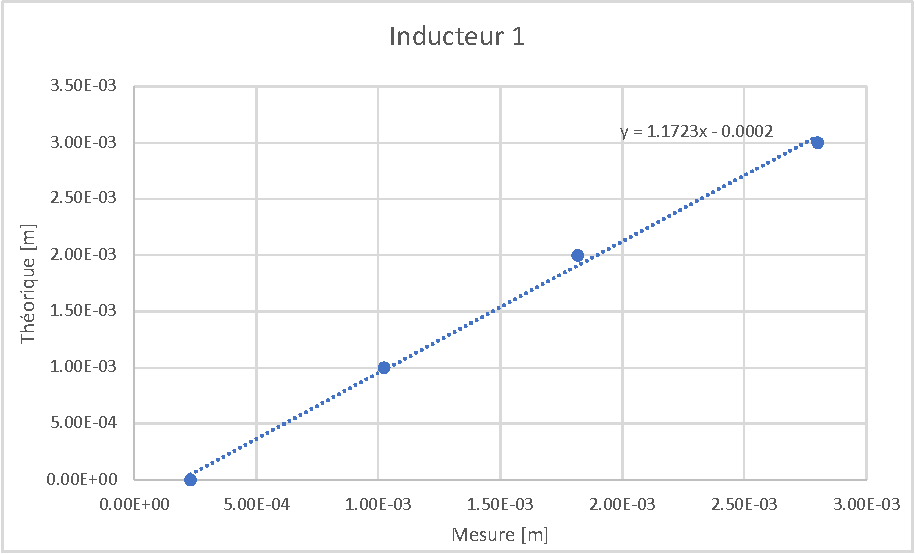
\includegraphics[width=1\linewidth]{assets/Chap3/PremEtaloInd1.pdf}
    \caption{Graphique de l'étalonnage de l'inducteur 1}
    \label{fig:Prem_tracé_ind1}
\end{figure}

\begin{figure}[H]
    \centering
    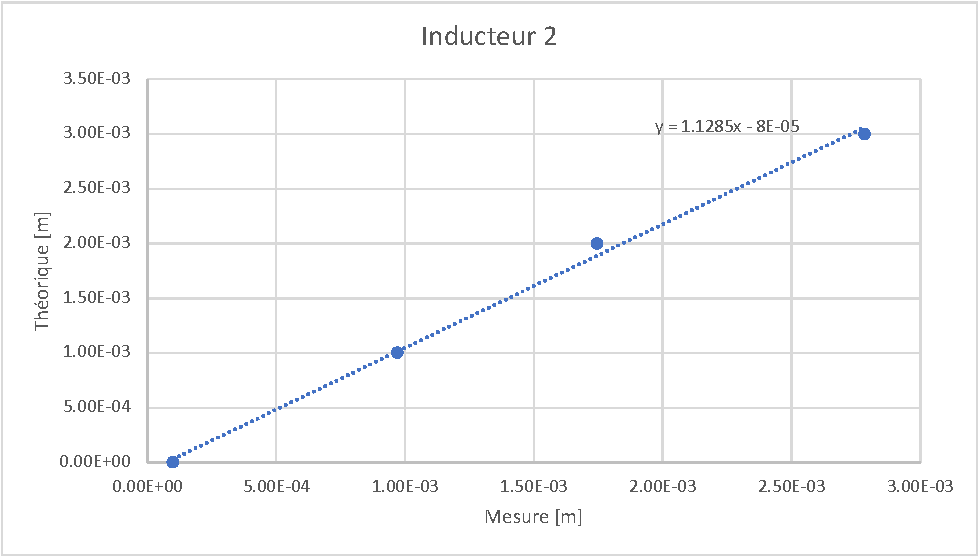
\includegraphics[width=1\linewidth]{assets/Chap3/PremEtaloInd2.pdf}
    \caption{Graphique de l'étalonnage de l'inducteur 2}
    \label{fig:Prem_tracé_ind2}
\end{figure}

\begin{figure}[H]
    \centering
    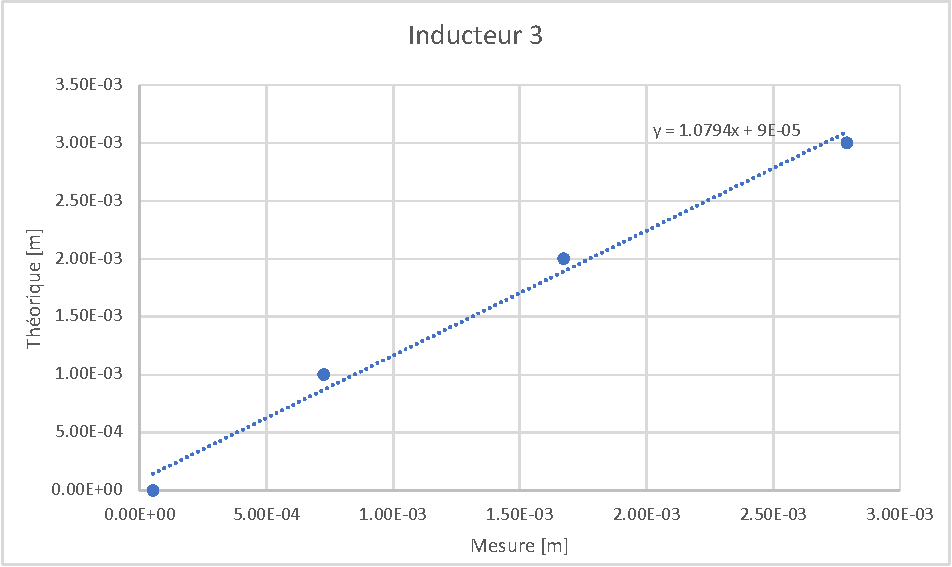
\includegraphics[width=1\linewidth]{assets/Chap3/PremEtaloInd3.pdf}
    \caption{Graphique de l'étalonnage de l'inducteur 3}
    \label{fig:Prem_tracé_ind3}
\end{figure}

\begin{figure}[H]
    \centering
    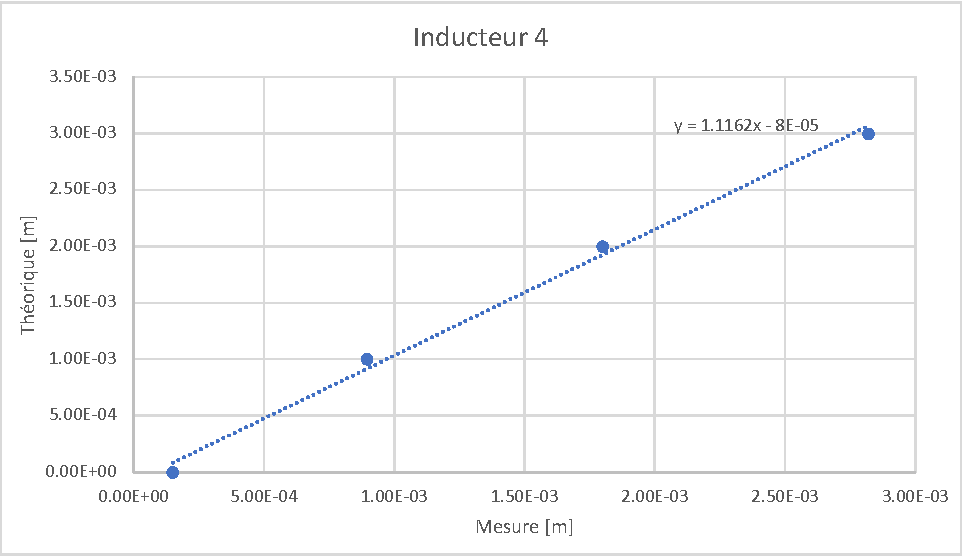
\includegraphics[width=1\linewidth]{assets/Chap3/PremEtaloInd4.pdf}
    \caption{Graphique de l'étalonnage de l'inducteur 4}
    \label{fig:Prem_tracé_ind4}
\end{figure}

L'analyse de ces tracés a permis de déduire des équations de correction intégrant un gain et un décalage (offset), où la variable $x$ représente la valeur issue de l'ADC convertie en millimètres.\\
Une vérification expérimentale a ensuite été menée, dont les résultats figurent dans le tableau \ref{tab:correction1_adc} :

\begin{table}[H]
    \centering
    \begin{tabular}{|c|c|c|c|c|}
        \hline
        \multicolumn{5}{|c|}{\textbf{Mesure des positions entrefers après l'ADC}}                     \\ \hline
        Inducteur          & Théorique {[}m{]} & Mesure {[}m{]} & Erreur   & Erreur relative {[}\%{]} \\ \hline
        \multirow{4}{*}{1} & 0.00E+00          & 1.81E-04       & 1.81E-04 & -                        \\ \cline{2-5}
                           & 1.00E-03          & 9.80E-04       & 2.00E-05 & 2.00                     \\ \cline{2-5}
                           & 2.00E-03          & 1.91E-03       & 9.10E-05 & 4.55                     \\ \cline{2-5}
                           & 3.00E-03          & 3.04E-03       & 3.90E-05 & 1.30                     \\ \hline
        \multirow{4}{*}{2} & 0.00E+00          & 1.70E-05       & 1.70E-05 & -                        \\ \cline{2-5}
                           & 1.00E-03          & 9.19E-04       & 8.10E-05 & 8.10                     \\ \cline{2-5}
                           & 2.00E-03          & 1.89E-03       & 1.07E-04 & 5.35                     \\ \cline{2-5}
                           & 3.00E-03          & 3.06E-03       & 5.80E-05 & 1.93                     \\ \hline
        \multirow{4}{*}{3} & 0.00E+00          & 1.08E-04       & 1.08E-04 & -                        \\ \cline{2-5}
                           & 1.00E-03          & 9.26E-04       & 7.40E-05 & 7.4                      \\ \cline{2-5}
                           & 2.00E-03          & 1.96E-03       & 3.70E-05 & 1.85                     \\ \cline{2-5}
                           & 3.00E-03          & 3.11E-03       & 1.09E-04 & 3.63                     \\ \hline
        \multirow{4}{*}{4} & 0.00E+00          & -1.00E-05      & 1.00E-05 & -                        \\ \cline{2-5}
                           & 1.00E-03          & 8.45E-04       & 1.55E-04 & 15.5                     \\ \cline{2-5}
                           & 2.00E-03          & 2.00E-03       & 5.00E-06 & 0.25                     \\ \cline{2-5}
                           & 3.00E-03          & 3.06E-03       & 6.10E-05 & 2.03                     \\ \hline
    \end{tabular}
    \caption{Erreurs de mesure des positions en sortie de l'ADC (1ère correction : application des courbes)}
    \label{tab:correction1_adc}
\end{table}

Malgré la faiblesse des erreurs relatives observées, l'implémentation de ces équations n'a pas apporté d'amélioration significative concernant la lévitation du système.

\subsection{Mesure après la calibration de tous les capteurs}
À la suite de l'étalonnage précédent, une calibration simultanée des quatre capteurs a été effectuée. L'objectif de cette démarche consistait à définir une origine de référence commune pour chaque inducteur :

\begin{figure}[H]
    \centering
    \includesvg[width=1\linewidth]{assets/Chap3/MaquetteCote}
    \caption{Méthode teachin en levant que l'avant}
    \label{fig:DessinMaquetteCote}
\end{figure}

Le schéma illustre le montage expérimental : le repère 7 désigne le support en bois, le repère 8 correspond à la carte principale et les repères 9 identifient les cartes de puissance.

Pour garantir une bonne homogénéité, les quatre inducteurs ont été soulevés puis abaissés selon la procédure détaillée dans la section \ref{sec:CalibrationCaptPos}.

À l'issue de cette calibration, une nouvelle série de mesures (sans correction) a été réalisée. Les données sont regroupées dans le tableau \ref{tab:recalib_sans_correction_adc} :

\begin{table}[H]
    \centering
    \begin{tabular}{|c|c|c|c|c|}
        \hline
        \multicolumn{5}{|c|}{\textbf{Mesure des positions entrefers après l'ADC}}                     \\ \hline
        Inducteur          & Théorique {[}m{]} & Mesure {[}m{]} & Erreur   & Erreur relative {[}\%{]} \\ \hline
        \multirow{4}{*}{1} & 0.00E+00          & 1.43E-04       & 1.43E-04 & -                        \\ \cline{2-5}
                           & 1.00E-03          & 8.23E-04       & 1.77E-04 & 17.7                     \\ \cline{2-5}
                           & 2.00E-03          & 1.79E-03       & 2.14E-04 & 10.7                     \\ \cline{2-5}
                           & 3.00E-03          & 2.80E-03       & 1.96E-04 & 6.53                     \\ \hline
        \multirow{4}{*}{2} & 0.00E+00          & 8.50E-05       & 8.50E-05 & -                        \\ \cline{2-5}
                           & 1.00E-03          & 8.66E-04       & 1.34E-04 & 13.4                     \\ \cline{2-5}
                           & 2.00E-03          & 1.87E-03       & 1.35E-04 & 6.75                     \\ \cline{2-5}
                           & 3.00E-03          & 2.83E-03       & 1.70E-04 & 5.67                     \\ \hline
        \multirow{4}{*}{3} & 0.00E+00          & 2.30E-05       & 2.30E-05 & -                        \\ \cline{2-5}
                           & 1.00E-03          & 7.09E-04       & 2.91E-04 & 29.1                     \\ \cline{2-5}
                           & 2.00E-03          & 1.69E-03       & 3.13E-04 & 15.65                    \\ \cline{2-5}
                           & 3.00E-03          & 2.80E-03       & 1.98E-04 & 6.6                      \\ \hline
        \multirow{4}{*}{4} & 0.00E+00          & 5.00E-05       & 5.00E-05 & -                        \\ \cline{2-5}
                           & 1.00E-03          & 8.13E-04       & 1.87E-04 & 18.7                     \\ \cline{2-5}
                           & 2.00E-03          & 1.74E-03       & 2.62E-04 & 13.1                     \\ \cline{2-5}
                           & 3.00E-03          & 2.82E-03       & 1.84E-04 & 6.13                     \\ \hline
    \end{tabular}
    \caption{Mesure des positions en sortie de l'ADC après recalibration complète et sans correction}
    \label{tab:recalib_sans_correction_adc}
\end{table}

Ces nouvelles données ont fait l'objet d'une modélisation graphique afin d'en déduire une fonction de correction à implémenter au sein du microcontrôleur. Les courbes obtenues sont visibles sur les figures \ref{fig:Sec_tracé_ind1}, \ref{fig:Sec_tracé_ind2}, \ref{fig:Sec_tracé_ind3} et \ref{fig:Sec_tracé_ind4} :

\begin{figure}[H]
    \centering
    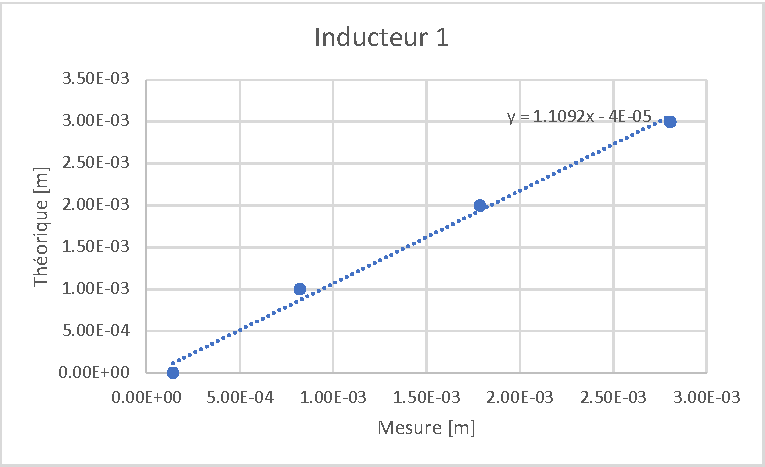
\includegraphics[width=1\linewidth]{assets/Chap3/SecEtaloInd1.pdf}
    \caption{Graphique du second étalonnage de l'inducteur 1}
    \label{fig:Sec_tracé_ind1}
\end{figure}

\begin{figure}[H]
    \centering
    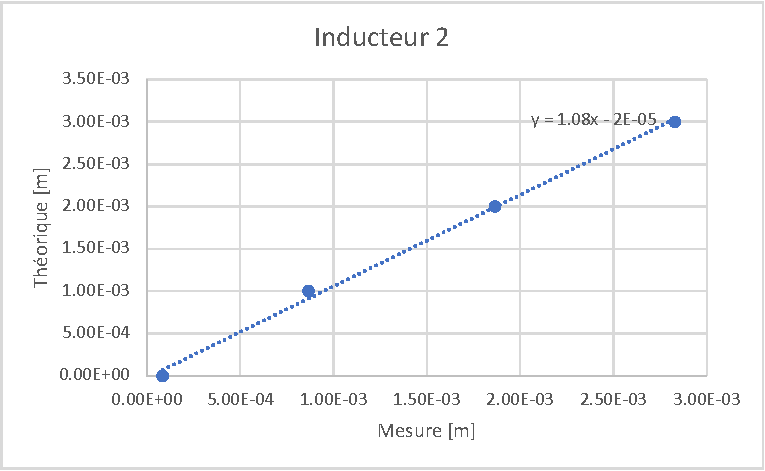
\includegraphics[width=1\linewidth]{assets/Chap3/SecEtaloInd2.pdf}
    \caption{Graphique du second étalonnage de l'inducteur 1}
    \label{fig:Sec_tracé_ind2}
\end{figure}

\begin{figure}[H]
    \centering
    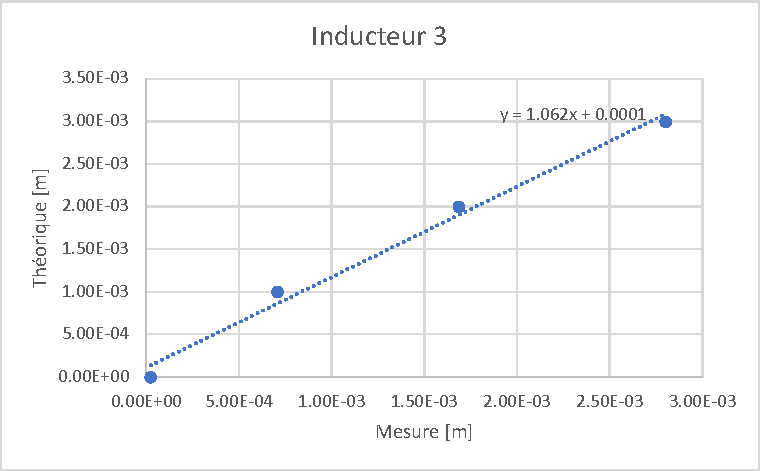
\includegraphics[width=1\linewidth]{assets/Chap3/SecEtaloInd3.pdf}
    \caption{Graphique du second étalonnage de l'inducteur 1}
    \label{fig:Sec_tracé_ind3}
\end{figure}

\begin{figure}[H]
    \centering
    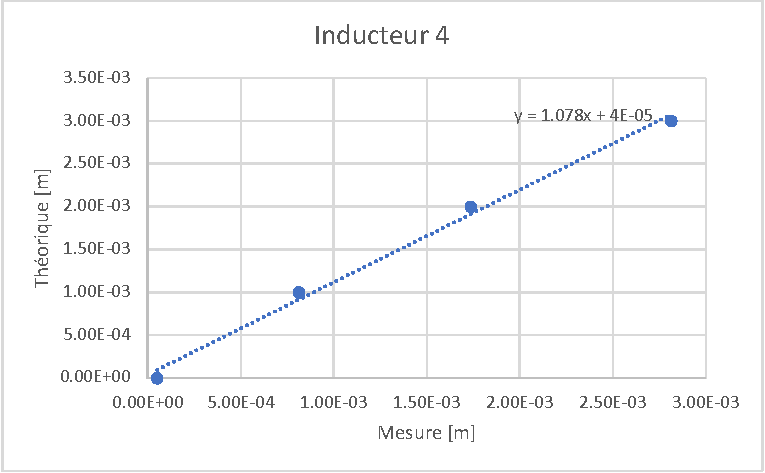
\includegraphics[width=1\linewidth]{assets/Chap3/SecEtaloInd4.pdf}
    \caption{Graphique du second étalonnage de l'inducteur 1}
    \label{fig:Sec_tracé_ind4}
\end{figure}

Après intégration de ces nouvelles équations dans le code source, une mesure de vérification a été effectuée. Les résultats sont présentés dans le tableau \ref{tab:verif_etalonnage_teachin_adc} :

\begin{table}[H]
    \centering
    \begin{tabular}{|c|c|c|c|c|}
        \hline
        \multicolumn{5}{|c|}{\textbf{Mesure des positions entrefers après l'ADC}}                     \\ \hline
        Inducteur          & Théorique {[}m{]} & Mesure {[}m{]} & Erreur   & Erreur relative {[}\%{]} \\ \hline
        \multirow{4}{*}{1} & 0.00E+00          & 1.06E-04       & 1.06E-04 & -                        \\ \cline{2-5}
                           & 1.00E-03          & 7.90E-04       & 2.10E-04 & 21                       \\ \cline{2-5}
                           & 2.00E-03          & 1.82E-03       & 1.85E-04 & 9.25                     \\ \cline{2-5}
                           & 3.00E-03          & 3.01E-03       & 1.10E-05 & 0.367                    \\ \hline
        \multirow{4}{*}{2} & 0.00E+00          & 9.30E-05       & 9.30E-05 & -                        \\ \cline{2-5}
                           & 1.00E-03          & 9.21E-04       & 7.90E-05 & 7.9                      \\ \cline{2-5}
                           & 2.00E-03          & 1.89E-03       & 1.06E-04 & 5.3                      \\ \cline{2-5}
                           & 3.00E-03          & 3.03E-03       & 2.80E-05 & 0.933                    \\ \hline
        \multirow{4}{*}{3} & 0.00E+00          & 1.38E-04       & 1.38E-04 & -                        \\ \cline{2-5}
                           & 1.00E-03          & 7.88E-04       & 2.12E-04 & 21.2                     \\ \cline{2-5}
                           & 2.00E-03          & 1.83E-03       & 1.74E-04 & 8.70                     \\ \cline{2-5}
                           & 3.00E-03          & 3.02E-03       & 1.50E-05 & 0.500                    \\ \hline
        \multirow{4}{*}{4} & 0.00E+00          & 1.16E-04       & 1.16E-04 & -                        \\ \cline{2-5}
                           & 1.00E-03          & 9.06E-04       & 9.40E-05 & 9.40                     \\ \cline{2-5}
                           & 2.00E-03          & 1.91E-03       & 8.70E-05 & 4.35                     \\ \cline{2-5}
                           & 3.00E-03          & 3.07E-03       & 7.30E-05 & 2.43                     \\ \hline
    \end{tabular}
    \caption{Mesure des positions en sortie de l'ADC (vérification de l'étalonnage après recalibration teach-in des 4 capteurs)}
    \label{tab:verif_etalonnage_teachin_adc}
\end{table}

Cependant, comme observé précédemment, ce nouvel étalonnage n'a pas permis d'améliorer la stabilité de la lévitation en conditions de fonctionnement.

\subsection{Mesure d'étalonnage des valeurs d'ADC}
\red{Remettre les tableaux de mesures car la valeur théorique était fausse}
Face à l'absence de résultats concluants, l'application d'une correction directe sur la valeur numérique de l'ADC a été testée. Lors des travaux antérieurs, la valeur brute de l'ADC était convertie par une simple règle de trois, formulée selon l'équation \ref{eq:conv_ADC_mm} :

\begin{equation}
    Conversion = \frac{Position\text{ }max - Position\text{ }min}{Valeur\text{ }max\text{ }de\text{ }l'adc}
    \label{eq:conv_ADC_mm}
\end{equation}

Avec :
\begin{itemize}
    \item Position maximale : 3~mm
    \item Position minimale : 0~mm
    \item Valeur maximale de l'ADC : 3722,7
\end{itemize}

Dans le but d'obtenir une correction plus précise et spécifique à chaque inducteur, une nouvelle fonction de transfert a été développée pour convertir directement le signal de l'ADC en une grandeur physique exprimée en millimètres.\\

Au cours des différentes campagnes d'essais, il a été constaté que les capteurs de position présentaient un comportement fortement non linéaire. L'utilisation d'une approximation linéaire classique a donc été écartée au profit d'une modélisation par régression polynomiale d'ordre supérieur. Les données brutes recueillies sont présentées dans les tableaux \ref{tab:adc_brut_inducteur1}, \ref{tab:adc_brut_inducteur2}, \ref{tab:adc_brut_inducteur3} et \ref{tab:adc_brut_inducteur4} :

\begin{table}[H]
    \centering
    \resizebox{\textwidth}{!}{%
        \begin{tabular}{|c|c|c|c|c|c|c|c|c|}
            \hline
            \multicolumn{9}{|c|}{\textbf{Mesure des positions brutes de l'ADC pour l'inducteur 1}}                                                                                                                                                                                                                                         \\ \hline
            Ligne              & Entrefer {[}m{]} & Théorique & \begin{tabular}[c]{@{}c@{}}Mesure\\ au centre\end{tabular} & \begin{tabular}[c]{@{}c@{}}Mesure\\ à gauche\end{tabular} & \begin{tabular}[c]{@{}c@{}}Mesure\\ à droite\end{tabular} & Moyenne & Erreur & \begin{tabular}[c]{@{}c@{}}Erreur\\ relative {[}\%{]}\end{tabular} \\ \hline
            \multirow{6}{*}{1} & 3.00E-03         & 3723      & 3492                                                       & 3490                                                      & 3492                                                      & 3492    & 231    & 6.20                                                               \\ \cline{2-9}
                               & 2.50E-03         & 2482      & 2599                                                       & 2699                                                      & 2568                                                      & 2622    & 140    & 5.64                                                               \\ \cline{2-9}
                               & 2.00E-03         & 1862      & 2096                                                       & 2171                                                      & 2040                                                      & 2103    & 241    & 12.9                                                               \\ \cline{2-9}
                               & 1.50E-03         & 1241      & 1467                                                       & 1552                                                      & 1379                                                      & 1466    & 225    & 18.1                                                               \\ \cline{2-9}
                               & 1.00E-03         & 621       & 747                                                        & 826                                                       & 703                                                       & 759     & 138    & 22.2                                                               \\ \cline{2-9}
                               & 0.00E+00         & 0         & 432                                                        & 527                                                       & 393                                                       & 451     & 451    & -                                                                  \\ \hline
            \multirow{6}{*}{2} & 3.00E-03         & 3723      & 3492                                                       & 3488                                                      & 3493                                                      & 3491    & 232    & 6.23                                                               \\ \cline{2-9}
                               & 2.50E-03         & 2482      & 2484                                                       & 2549                                                      & 2451                                                      & 2495    & 13     & 0.524                                                              \\ \cline{2-9}
                               & 2.00E-03         & 1862      & 2025                                                       & 2074                                                      & 1976                                                      & 2025    & 163    & 8.75                                                               \\ \cline{2-9}
                               & 1.50E-03         & 1241      & 1350                                                       & 1429                                                      & 1321                                                      & 1367    & 126    & 10.2                                                               \\ \cline{2-9}
                               & 1.00E-03         & 621       & 699                                                        & 743                                                       & 650                                                       & 698     & 77     & 12.4                                                               \\ \cline{2-9}
                               & 0.00E+00         & 0         & 321                                                        & 401                                                       & 261                                                       & 328     & 328    & -                                                                  \\ \hline
            \multirow{6}{*}{3} & 3.00E-03         & 3723      & 3491                                                       & 3488                                                      & 3488                                                      & 3489    & 234    & 6.29                                                               \\ \cline{2-9}
                               & 2.50E-03         & 2482      & 2423                                                       & 2315                                                      & 2419                                                      & 2386    & 96     & 3.87                                                               \\ \cline{2-9}
                               & 2.00E-03         & 1862      & 1902                                                       & 1903                                                      & 1874                                                      & 1893    & 31     & 1.66                                                               \\ \cline{2-9}
                               & 1.50E-03         & 1241      & 1199                                                       & 1216                                                      & 1187                                                      & 1201    & 40     & 3.22                                                               \\ \cline{2-9}
                               & 1.00E-03         & 621       & 476                                                        & 522                                                       & 465                                                       & 488     & 133    & 21.4                                                               \\ \cline{2-9}
                               & 0.00E+00         & 0         & 230                                                        & 221                                                       & 162                                                       & 205     & 205    & -                                                                  \\ \hline
            \multirow{6}{*}{4} & 3.00E-03         & 3723      & 3486                                                       & 3483                                                      & 3492                                                      & 3487    & 236    & 6.34                                                               \\ \cline{2-9}
                               & 2.50E-03         & 2482      & 2452                                                       & 2417                                                      & 2410                                                      & 2427    & 55     & 2.22                                                               \\ \cline{2-9}
                               & 2.00E-03         & 1862      & 1903                                                       & 1912                                                      & 1851                                                      & 1889    & 27     & 1.45                                                               \\ \cline{2-9}
                               & 1.50E-03         & 1241      & 1264                                                       & 1292                                                      & 1193                                                      & 1250    & 9      & 0.725                                                              \\ \cline{2-9}
                               & 1.00E-03         & 621       & 494                                                        & 507                                                       & 453                                                       & 485     & 136    & 21.9                                                               \\ \cline{2-9}
                               & 0.00E+00         & 0         & 148                                                        & 186                                                       & 142                                                       & 159     & 159    & -                                                                  \\ \hline
            \multirow{6}{*}{5} & 3.00E-03         & 3723      & 3486                                                       & 3485                                                      & 3489                                                      & 3487    & 236    & 6.34                                                               \\ \cline{2-9}
                               & 2.50E-03         & 2482      & 2496                                                       & 2527                                                      & 2515                                                      & 2513    & 31     & 1.25                                                               \\ \cline{2-9}
                               & 2.00E-03         & 1862      & 1969                                                       & 1997                                                      & 1881                                                      & 1949    & 87     & 4.67                                                               \\ \cline{2-9}
                               & 1.50E-03         & 1241      & 1300                                                       & 1367                                                      & 1196                                                      & 1288    & 47     & 3.79                                                               \\ \cline{2-9}
                               & 1.00E-03         & 621       & 518                                                        & 599                                                       & 572                                                       & 563     & 58     & 9.34                                                               \\ \cline{2-9}
                               & 0.00E+00         & 0         & 277                                                        & 341                                                       & 243                                                       & 287     & 287    & -                                                                  \\ \hline
        \end{tabular}%
    }
    \caption{Mesure des positions brutes de l'ADC pour l'inducteur 1}
    \label{tab:adc_brut_inducteur1}
\end{table}

\begin{table}[H]
    \centering
    \resizebox{\textwidth}{!}{%
        \begin{tabular}{|c|c|c|c|c|c|c|c|c|}
            \hline
            \multicolumn{9}{|c|}{\textbf{Mesure des positions brutes de l'ADC pour l'inducteur 2}}                                                                                                                                                                                                                                         \\ \hline
            Ligne              & Entrefer {[}m{]} & Théorique & \begin{tabular}[c]{@{}c@{}}Mesure\\ au centre\end{tabular} & \begin{tabular}[c]{@{}c@{}}Mesure\\ à gauche\end{tabular} & \begin{tabular}[c]{@{}c@{}}Mesure\\ à droite\end{tabular} & Moyenne & Erreur & \begin{tabular}[c]{@{}c@{}}Erreur\\ relative {[}\%{]}\end{tabular} \\ \hline
            \multirow{6}{*}{1} & 3.00E-03         & 3723      & 3518                                                       & 3518                                                      & 3518                                                      & 3518    & 205    & 5.51                                                               \\ \cline{2-9}
                               & 2.50E-03         & 2482      & 2441                                                       & 2388                                                      & 2521                                                      & 2450    & 32     & 1.29                                                               \\ \cline{2-9}
                               & 2.00E-03         & 1862      & 1907                                                       & 1849                                                      & 1931                                                      & 1896    & 34     & 1.83                                                               \\ \cline{2-9}
                               & 1.50E-03         & 1241      & 1291                                                       & 1261                                                      & 1340                                                      & 1298    & 57     & 4.59                                                               \\ \cline{2-9}
                               & 1.00E-03         & 621       & 609                                                        & 550                                                       & 681                                                       & 614     & 7      & 1.13                                                               \\ \cline{2-9}
                               & 0.00E+00         & 0         & 317                                                        & 247                                                       & 354                                                       & 306     & 306    & -                                                                  \\ \hline
            \multirow{6}{*}{2} & 3.00E-03         & 3723      & 3518                                                       & 3518                                                      & 3518                                                      & 3518    & 205    & 5.51                                                               \\ \cline{2-9}
                               & 2.50E-03         & 2482      & 2358                                                       & 2281                                                      & 2390                                                      & 2343    & 139    & 5.60                                                               \\ \cline{2-9}
                               & 2.00E-03         & 1862      & 1843                                                       & 1778                                                      & 1888                                                      & 1837    & 25     & 1.34                                                               \\ \cline{2-9}
                               & 1.50E-03         & 1241      & 1248                                                       & 1196                                                      & 1281                                                      & 1242    & 1      & 0.0806                                                             \\ \cline{2-9}
                               & 1.00E-03         & 621       & 579                                                        & 496                                                       & 643                                                       & 573     & 48     & 7.73                                                               \\ \cline{2-9}
                               & 0.00E+00         & 0         & 204                                                        & 104                                                       & 233                                                       & 181     & 181    & -                                                                  \\ \hline
            \multirow{6}{*}{3} & 3.00E-03         & 3723      & 3518                                                       & 3518                                                      & 3518                                                      & 3518    & 205    & 5.51                                                               \\ \cline{2-9}
                               & 2.50E-03         & 2482      & 2443                                                       & 2316                                                      & 2499                                                      & 2420    & 62     & 2.50                                                               \\ \cline{2-9}
                               & 2.00E-03         & 1862      & 1871                                                       & 1788                                                      & 1913                                                      & 1858    & 4      & 0.215                                                              \\ \cline{2-9}
                               & 1.50E-03         & 1241      & 1231                                                       & 1147                                                      & 1277                                                      & 1219    & 22     & 1.77                                                               \\ \cline{2-9}
                               & 1.00E-03         & 621       & 503                                                        & 463                                                       & 586                                                       & 518     & 103    & 16.6                                                               \\ \cline{2-9}
                               & 0.00E+00         & 0         & 148                                                        & 59                                                        & 239                                                       & 149     & 149    & -                                                                  \\ \hline
            \multirow{6}{*}{4} & 3.00E-03         & 3723      & 3518                                                       & 3518                                                      & 3518                                                      & 3518    & 205    & 5.51                                                               \\ \cline{2-9}
                               & 2.50E-03         & 2482      & 2486                                                       & 2428                                                      & 2635                                                      & 2517    & 35     & 1.41                                                               \\ \cline{2-9}
                               & 2.00E-03         & 1862      & 1997                                                       & 1945                                                      & 2078                                                      & 2007    & 145    & 7.79                                                               \\ \cline{2-9}
                               & 1.50E-03         & 1241      & 1361                                                       & 1294                                                      & 1432                                                      & 1363    & 122    & 9.83                                                               \\ \cline{2-9}
                               & 1.00E-03         & 621       & 630                                                        & 568                                                       & 734                                                       & 644     & 23     & 3.70                                                               \\ \cline{2-9}
                               & 0.00E+00         & 0         & 149                                                        & 62                                                        & 230                                                       & 147     & 147    & -                                                                  \\ \hline
            \multirow{6}{*}{5} & 3.00E-03         & 3723      & 3518                                                       & 3518                                                      & 3518                                                      & 3518    & 205    & 5.51                                                               \\ \cline{2-9}
                               & 2.50E-03         & 2482      & 2478                                                       & 2428                                                      & 2422                                                      & 2443    & 39     & 1.57                                                               \\ \cline{2-9}
                               & 2.00E-03         & 1862      & 1938                                                       & 1890                                                      & 2043                                                      & 1957    & 95     & 5.10                                                               \\ \cline{2-9}
                               & 1.50E-03         & 1241      & 1375                                                       & 1293                                                      & 1420                                                      & 1363    & 122    & 9.83                                                               \\ \cline{2-9}
                               & 1.00E-03         & 621       & 620                                                        & 586                                                       & 541                                                       & 583     & 38     & 6.12                                                               \\ \cline{2-9}
                               & 0.00E+00         & 0         & 269                                                        & 228                                                       & 284                                                       & 261     & 261    & -                                                                  \\ \hline
        \end{tabular}%
    }
    \caption{Mesure des positions brutes de l'ADC pour l'inducteur 2}
    \label{tab:adc_brut_inducteur2}
\end{table}

\begin{table}[H]
    \centering
    \resizebox{\textwidth}{!}{%
        \begin{tabular}{|c|c|c|c|c|c|c|c|c|}
            \hline
            \multicolumn{9}{|c|}{\textbf{Mesure des positions brutes de l'ADC pour l'inducteur 3}}                                                                                                                                                                                                                                         \\ \hline
            Ligne              & Entrefer {[}m{]} & Théorique & \begin{tabular}[c]{@{}c@{}}Mesure\\ au centre\end{tabular} & \begin{tabular}[c]{@{}c@{}}Mesure\\ à gauche\end{tabular} & \begin{tabular}[c]{@{}c@{}}Mesure\\ à droite\end{tabular} & Moyenne & Erreur & \begin{tabular}[c]{@{}c@{}}Erreur\\ relative {[}\%{]}\end{tabular} \\ \hline
            \multirow{6}{*}{1} & 3.00E-03         & 3723      & 3486                                                       & 3486                                                      & 3486                                                      & 3486    & 237    & 6.37                                                               \\ \cline{2-9}
                               & 2.50E-03         & 2482      & 2385                                                       & 2475                                                      & 2333                                                      & 2398    & 84     & 3.38                                                               \\ \cline{2-9}
                               & 2.00E-03         & 1862      & 1811                                                       & 1914                                                      & 1779                                                      & 1835    & 27     & 1.45                                                               \\ \cline{2-9}
                               & 1.50E-03         & 1241      & 1206                                                       & 1226                                                      & 1127                                                      & 1187    & 54     & 4.35                                                               \\ \cline{2-9}
                               & 1.00E-03         & 621       & 506                                                        & 502                                                       & 467                                                       & 492     & 129    & 20.8                                                               \\ \cline{2-9}
                               & 0.00E+00         & 0         & 104                                                        & 40                                                        & 106                                                       & 84      & 84     & -                                                                  \\ \hline
            \multirow{6}{*}{2} & 3.00E-03         & 3723      & 3487                                                       & 3487                                                      & 3487                                                      & 3487    & 236    & 6.34                                                               \\ \cline{2-9}
                               & 2.50E-03         & 2482      & 2230                                                       & 2265                                                      & 2208                                                      & 2235    & 247    & 9.95                                                               \\ \cline{2-9}
                               & 2.00E-03         & 1862      & 1651                                                       & 1706                                                      & 1615                                                      & 1658    & 204    & 11.0                                                               \\ \cline{2-9}
                               & 1.50E-03         & 1241      & 1053                                                       & 1071                                                      & 990                                                       & 1038    & 203    & 16.4                                                               \\ \cline{2-9}
                               & 1.00E-03         & 621       & 237                                                        & 274                                                       & 198                                                       & 237     & 384    & 61.8                                                               \\ \cline{2-9}
                               & 0.00E+00         & 0         & 27                                                         & 20                                                        & 29                                                        & 26      & 26     & -                                                                  \\ \hline
            \multirow{6}{*}{3} & 3.00E-03         & 3723      & 3486                                                       & 3487                                                      & 3487                                                      & 3487    & 236    & 6.34                                                               \\ \cline{2-9}
                               & 2.50E-03         & 2482      & 2111                                                       & 2153                                                      & 2117                                                      & 2127    & 355    & 14.30                                                              \\ \cline{2-9}
                               & 2.00E-03         & 1862      & 1657                                                       & 1666                                                      & 1600                                                      & 1641    & 221    & 11.87                                                              \\ \cline{2-9}
                               & 1.50E-03         & 1241      & 972                                                        & 962                                                       & 982                                                       & 972     & 269    & 21.68                                                              \\ \cline{2-9}
                               & 1.00E-03         & 621       & 264                                                        & 299                                                       & 250                                                       & 271     & 350    & 56.4                                                               \\ \cline{2-9}
                               & 0.00E+00         & 0         & 52                                                         & 18                                                        & 30                                                        & 34      & 34     & -                                                                  \\ \hline
            \multirow{6}{*}{4} & 3.00E-03         & 3723      & 3487                                                       & 3487                                                      & 3474                                                      & 3483    & 240    & 6.45                                                               \\ \cline{2-9}
                               & 2.50E-03         & 2482      & 2289                                                       & 2359                                                      & 2195                                                      & 2281    & 201    & 8.10                                                               \\ \cline{2-9}
                               & 2.00E-03         & 1862      & 1736                                                       & 1811                                                      & 1649                                                      & 1732    & 130    & 6.98                                                               \\ \cline{2-9}
                               & 1.50E-03         & 1241      & 1123                                                       & 1182                                                      & 977                                                       & 1094    & 147    & 11.8                                                               \\ \cline{2-9}
                               & 1.00E-03         & 621       & 362                                                        & 431                                                       & 300                                                       & 365     & 256    & 41.2                                                               \\ \cline{2-9}
                               & 0.00E+00         & 0         & 142                                                        & 126                                                       & 98                                                        & 122     & 122    & -                                                                  \\ \hline
            \multirow{6}{*}{5} & 3.00E-03         & 3723      & 3487                                                       & 3487                                                      & 3487                                                      & 3487    & 236    & 6.34                                                               \\ \cline{2-9}
                               & 2.50E-03         & 2482      & 2340                                                       & 2425                                                      & 2407                                                      & 2391    & 91     & 3.67                                                               \\ \cline{2-9}
                               & 2.00E-03         & 1862      & 1855                                                       & 1919                                                      & 1780                                                      & 1852    & 10     & 0.537                                                              \\ \cline{2-9}
                               & 1.50E-03         & 1241      & 1173                                                       & 1261                                                      & 1120                                                      & 1185    & 56     & 4.51                                                               \\ \cline{2-9}
                               & 1.00E-03         & 621       & 487                                                        & 587                                                       & 545                                                       & 540     & 81     & 13.0                                                               \\ \cline{2-9}
                               & 0.00E+00         & 0         & 281                                                        & 266                                                       & 225                                                       & 258     & 258    & -                                                                  \\ \hline
        \end{tabular}%
    }
    \caption{Mesure des positions brutes de l'ADC pour l'inducteur 3}
    \label{tab:adc_brut_inducteur3}
\end{table}

\begin{table}[H]
    \centering
    \resizebox{\textwidth}{!}{%
        \begin{tabular}{|c|c|c|c|c|c|c|c|c|}
            \hline
            \multicolumn{9}{|c|}{\textbf{Mesure des positions brutes de l'ADC pour l'inducteur 4}}                                                                                                                                                                                                                                         \\ \hline
            Ligne              & Entrefer {[}m{]} & Théorique & \begin{tabular}[c]{@{}c@{}}Mesure\\ au centre\end{tabular} & \begin{tabular}[c]{@{}c@{}}Mesure\\ à gauche\end{tabular} & \begin{tabular}[c]{@{}c@{}}Mesure\\ à droite\end{tabular} & Moyenne & Erreur & \begin{tabular}[c]{@{}c@{}}Erreur\\ relative {[}\%{]}\end{tabular} \\ \hline
            \multirow{6}{*}{1} & 3.00E-03         & 3723      & 3509                                                       & 3477                                                      & 3509                                                      & 3499    & 224    & 6.02                                                               \\ \cline{2-9}
                               & 2.50E-03         & 2482      & 2379                                                       & 2323                                                      & 2453                                                      & 2385    & 97     & 3.91                                                               \\ \cline{2-9}
                               & 2.00E-03         & 1862      & 1867                                                       & 1803                                                      & 1952                                                      & 1874    & 12     & 0.644                                                              \\ \cline{2-9}
                               & 1.50E-03         & 1241      & 1240                                                       & 1168                                                      & 1285                                                      & 1231    & 10     & 0.806                                                              \\ \cline{2-9}
                               & 1.00E-03         & 621       & 547                                                        & 485                                                       & 634                                                       & 556     & 65     & 10.5                                                               \\ \cline{2-9}
                               & 0.00E+00         & 0         & 18                                                         & 14                                                        & 98                                                        & 44      & 44     & -                                                                  \\ \hline
            \multirow{6}{*}{2} & 3.00E-03         & 3723      & 3496                                                       & 3436                                                      & 3509                                                      & 3481    & 242    & 6.50                                                               \\ \cline{2-9}
                               & 2.50E-03         & 2482      & 2342                                                       & 2271                                                      & 2330                                                      & 2315    & 167    & 6.73                                                               \\ \cline{2-9}
                               & 2.00E-03         & 1862      & 1806                                                       & 1724                                                      & 1847                                                      & 1793    & 69     & 3.71                                                               \\ \cline{2-9}
                               & 1.50E-03         & 1241      & 1148                                                       & 1096                                                      & 1186                                                      & 1144    & 97     & 7.82                                                               \\ \cline{2-9}
                               & 1.00E-03         & 621       & 440                                                        & 387                                                       & 503                                                       & 444     & 177    & 28.5                                                               \\ \cline{2-9}
                               & 0.00E+00         & 0         & 14                                                         & 13                                                        & 64                                                        & 31      & 31     & -                                                                  \\ \hline
            \multirow{6}{*}{3} & 3.00E-03         & 3723      & 3484                                                       & 3424                                                      & 3432                                                      & 3447    & 276    & 7.41                                                               \\ \cline{2-9}
                               & 2.50E-03         & 2482      & 2285                                                       & 2231                                                      & 2332                                                      & 2283    & 199    & 8.02                                                               \\ \cline{2-9}
                               & 2.00E-03         & 1862      & 1776                                                       & 1701                                                      & 1815                                                      & 1764    & 98     & 5.26                                                               \\ \cline{2-9}
                               & 1.50E-03         & 1241      & 1117                                                       & 1056                                                      & 1210                                                      & 1128    & 113    & 9.11                                                               \\ \cline{2-9}
                               & 1.00E-03         & 621       & 459                                                        & 406                                                       & 533                                                       & 466     & 155    & 25.0                                                               \\ \cline{2-9}
                               & 0.00E+00         & 0         & 15                                                         & 13                                                        & 127                                                       & 52      & 52     & -                                                                  \\ \hline
            \multirow{6}{*}{4} & 3.00E-03         & 3723      & 3402                                                       & 3342                                                      & 3498                                                      & 3414    & 309    & 8.30                                                               \\ \cline{2-9}
                               & 2.50E-03         & 2482      & 2216                                                       & 2177                                                      & 2301                                                      & 2232    & 250    & 10.07                                                              \\ \cline{2-9}
                               & 2.00E-03         & 1862      & 1694                                                       & 1604                                                      & 1774                                                      & 1691    & 171    & 9.18                                                               \\ \cline{2-9}
                               & 1.50E-03         & 1241      & 1043                                                       & 1011                                                      & 1134                                                      & 1063    & 178    & 14.34                                                              \\ \cline{2-9}
                               & 1.00E-03         & 621       & 370                                                        & 296                                                       & 490                                                       & 386     & 235    & 37.8                                                               \\ \cline{2-9}
                               & 0.00E+00         & 0         & 38                                                         & 20                                                        & 139                                                       & 66      & 66     & -                                                                  \\ \hline
            \multirow{6}{*}{5} & 3.00E-03         & 3723      & 3400                                                       & 3361                                                      & 3443                                                      & 3402    & 321    & 8.62                                                               \\ \cline{2-9}
                               & 2.50E-03         & 2482      & 2203                                                       & 2124                                                      & 2149                                                      & 2159    & 323    & 13.01                                                              \\ \cline{2-9}
                               & 2.00E-03         & 1862      & 1672                                                       & 1592                                                      & 1758                                                      & 1674    & 188    & 10.10                                                              \\ \cline{2-9}
                               & 1.50E-03         & 1241      & 1045                                                       & 996                                                       & 1078                                                      & 1040    & 201    & 16.20                                                              \\ \cline{2-9}
                               & 1.00E-03         & 621       & 522                                                        & 412                                                       & 433                                                       & 456     & 165    & 26.6                                                               \\ \cline{2-9}
                               & 0.00E+00         & 0         & 29                                                         & 28                                                        & 26                                                        & 28      & 28     & -                                                                  \\ \hline
        \end{tabular}%
    }
    \caption{Mesure des positions brutes de l'ADC pour l'inducteur 4}
    \label{tab:adc_brut_inducteur4}
\end{table}

Une moyenne de ces valeurs a ensuite été calculée pour chaque point de mesure, aboutissant aux résultats du tableau \ref{tab:adc_brut_moyenne} :

\begin{table}[H]
    \centering
    \begin{tabular}{|c|c|c|c|c|c|}
        \hline
        \multicolumn{6}{|c|}{\textbf{Mesure des positions de l'ADC moyenné}}                                                                      \\ \hline
        Inducteur          & Entrefer {[}m{]} & Théorique & Moyenne & Erreur & \begin{tabular}[c]{@{}c@{}}Erreur\\ relative {[}\%{]}\end{tabular} \\ \hline
        \multirow{6}{*}{1} & 3.00E-03         & 3723      & 3489    & 234    & 6.29                                                               \\ \cline{2-6}
                           & 2.50E-03         & 2482      & 2489    & 7      & 0.28                                                               \\ \cline{2-6}
                           & 2.00E-03         & 1862      & 1972    & 110    & 5.91                                                               \\ \cline{2-6}
                           & 1.50E-03         & 1241      & 1315    & 74     & 5.96                                                               \\ \cline{2-6}
                           & 1.00E-03         & 621       & 599     & 22     & 3.54                                                               \\ \cline{2-6}
                           & 0.00E+00         & 0         & 286     & 286    & -                                                                  \\ \hline
        \multirow{6}{*}{2} & 3.00E-03         & 3723      & 3518    & 205    & 5.51                                                               \\ \cline{2-6}
                           & 2.50E-03         & 2482      & 2435    & 47     & 1.89                                                               \\ \cline{2-6}
                           & 2.00E-03         & 1862      & 1911    & 49     & 2.63                                                               \\ \cline{2-6}
                           & 1.50E-03         & 1241      & 1297    & 56     & 4.51                                                               \\ \cline{2-6}
                           & 1.00E-03         & 621       & 586     & 35     & 5.64                                                               \\ \cline{2-6}
                           & 0.00E+00         & 0         & 209     & 209    & -                                                                  \\ \hline
        \multirow{6}{*}{3} & 3.00E-03         & 3723      & 3486    & 237    & 6.37                                                               \\ \cline{2-6}
                           & 2.50E-03         & 2482      & 2287    & 195    & 7.86                                                               \\ \cline{2-6}
                           & 2.00E-03         & 1862      & 1744    & 118    & 6.34                                                               \\ \cline{2-6}
                           & 1.50E-03         & 1241      & 1095    & 146    & 11.76                                                              \\ \cline{2-6}
                           & 1.00E-03         & 621       & 381     & 240    & 38.6                                                               \\ \cline{2-6}
                           & 0.00E+00         & 0         & 105     & 105    & -                                                                  \\ \hline
        \multirow{6}{*}{4} & 3.00E-03         & 3723      & 3449    & 274    & 7.36                                                               \\ \cline{2-6}
                           & 2.50E-03         & 2482      & 2275    & 207    & 8.34                                                               \\ \cline{2-6}
                           & 2.00E-03         & 1862      & 1759    & 103    & 5.53                                                               \\ \cline{2-6}
                           & 1.50E-03         & 1241      & 1121    & 120    & 9.67                                                               \\ \cline{2-6}
                           & 1.00E-03         & 621       & 462     & 159    & 25.6                                                               \\ \cline{2-6}
                           & 0.00E+00         & 0         & 44      & 44     & -                                                                  \\ \hline
    \end{tabular}
    \caption{Mesure des positions de l'ADC moyenné}
    \label{tab:adc_brut_moyenne}
\end{table}

Afin d'implémenter des équations d'ordre supérieur de manière optimale, la méthode de Horner \cite{Horner} a été employée, comme défini dans l'équation \ref{eq:Horner} :

\begin{equation}
    y = ((a_5 \cdot x + a_4) \cdot x + a_3) \cdot x + a_2) \cdot x + a_1) \cdot x + a_0
    \label{eq:Horner}
\end{equation}

Pour un polynôme d'ordre inférieur, tel qu'un ordre 3, les coefficients $a_5$ et $a_4$ sont nuls.

Une première tentative a été réalisée à l'aide d'un polynôme d'ordre 5. Les courbes correspondantes sont représentées sur les figures \ref{fig:Ind1Pol5}, \ref{fig:Ind2Pol5}, \ref{fig:Ind3Pol5} et \ref{fig:Ind4Pol5} :

\begin{figure}[H]
    \centering
    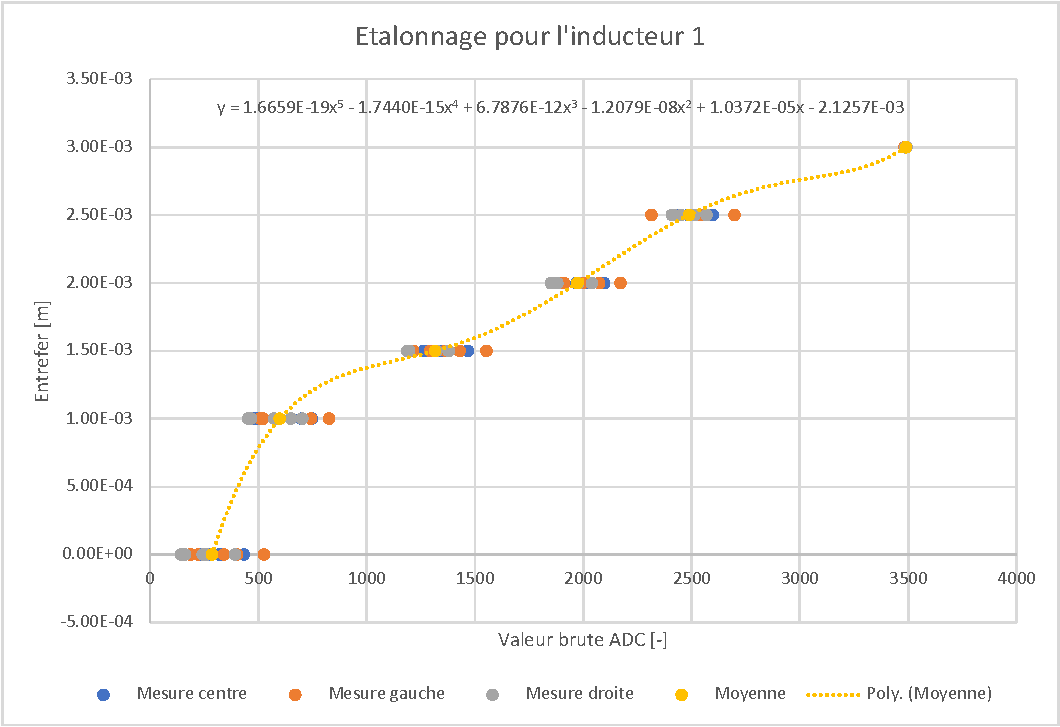
\includegraphics[width=1\linewidth]{assets/Chap3/EtaADCPol5/EtaADCPol5-1.pdf}
    \caption{Graphique d'étalonnage de l'ADC de l'inducteur 1 (polynome d'ordre 5)}
    \label{fig:Ind1Pol5}
\end{figure}

\begin{figure}[H]
    \centering
    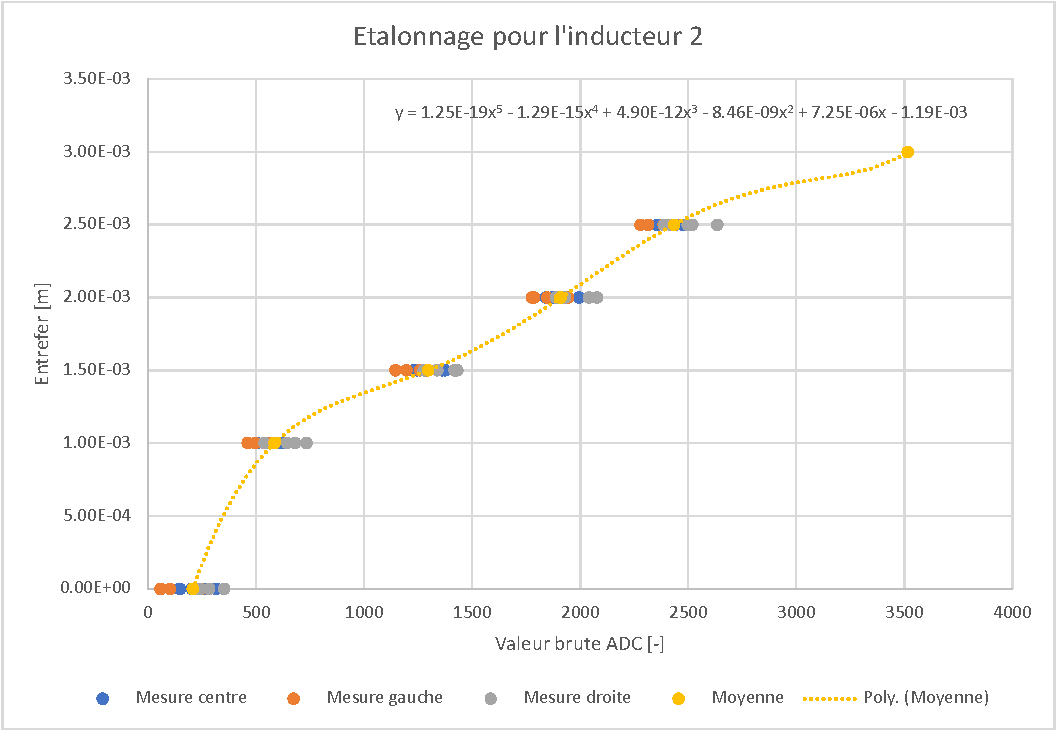
\includegraphics[width=1\linewidth]{assets/Chap3/EtaADCPol5/EtaADCPol5-2.pdf}
    \caption{Graphique d'étalonnage de l'ADC de l'inducteur 2 (polynome d'ordre 5)}
    \label{fig:Ind2Pol5}
\end{figure}

\begin{figure}[H]
    \centering
    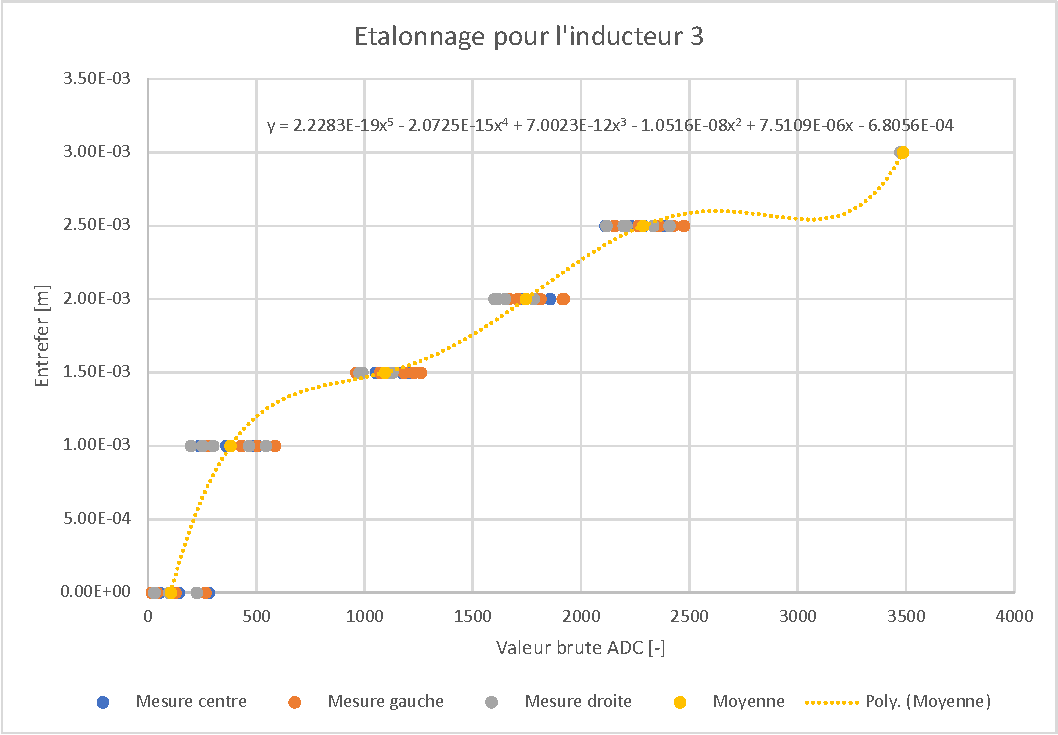
\includegraphics[width=1\linewidth]{assets/Chap3/EtaADCPol5/EtaADCPol5-3.pdf}
    \caption{Graphique d'étalonnage de l'ADC de l'inducteur 3 (polynome d'ordre 5)}
    \label{fig:Ind3Pol5}
\end{figure}

\begin{figure}[H]
    \centering
    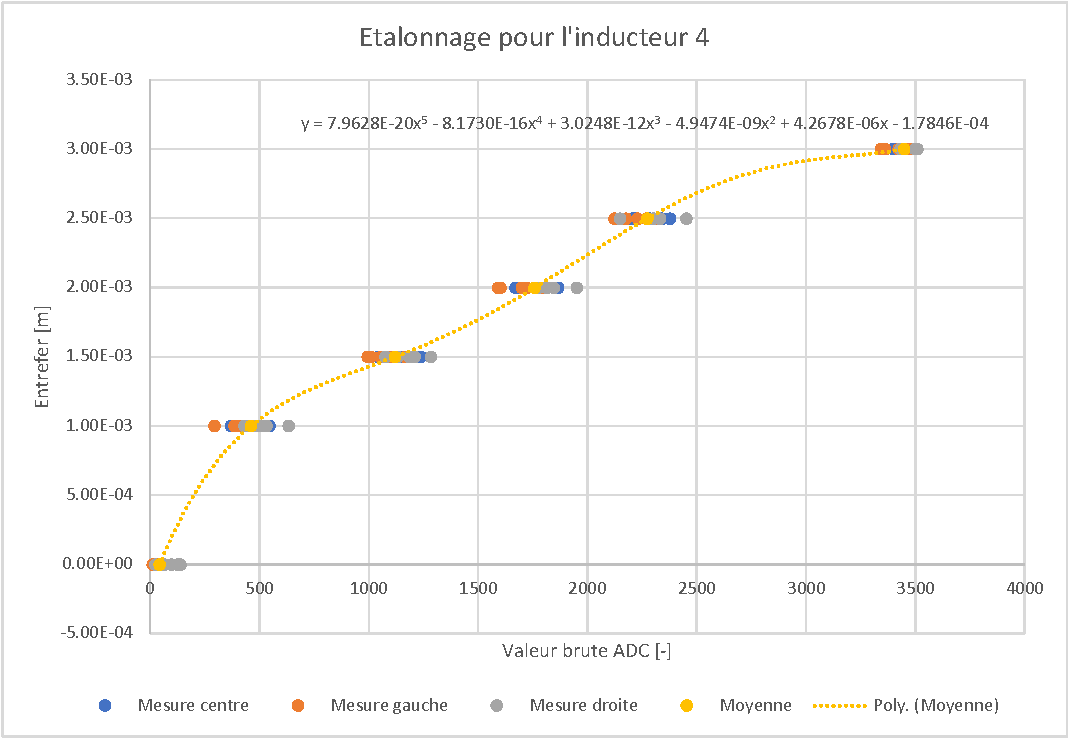
\includegraphics[width=1\linewidth]{assets/Chap3/EtaADCPol5/EtaADCPol5-4.pdf}
    \caption{Graphique d'étalonnage de l'ADC de l'inducteur 4 (polynome d'ordre 5)}
    \label{fig:Ind4Pol5}
\end{figure}

Ces modélisations n'étant pas concluantes et semblant restreindre la dynamique du système, le degré du polynôme a été réduit à 3. Cette approche a généré les tracés des figures \ref{fig:Ind1Pol3}, \ref{fig:Ind2Pol3}, \ref{fig:Ind3Pol3} et \ref{fig:Ind4Pol3} :

\begin{figure}[H]
    \centering
    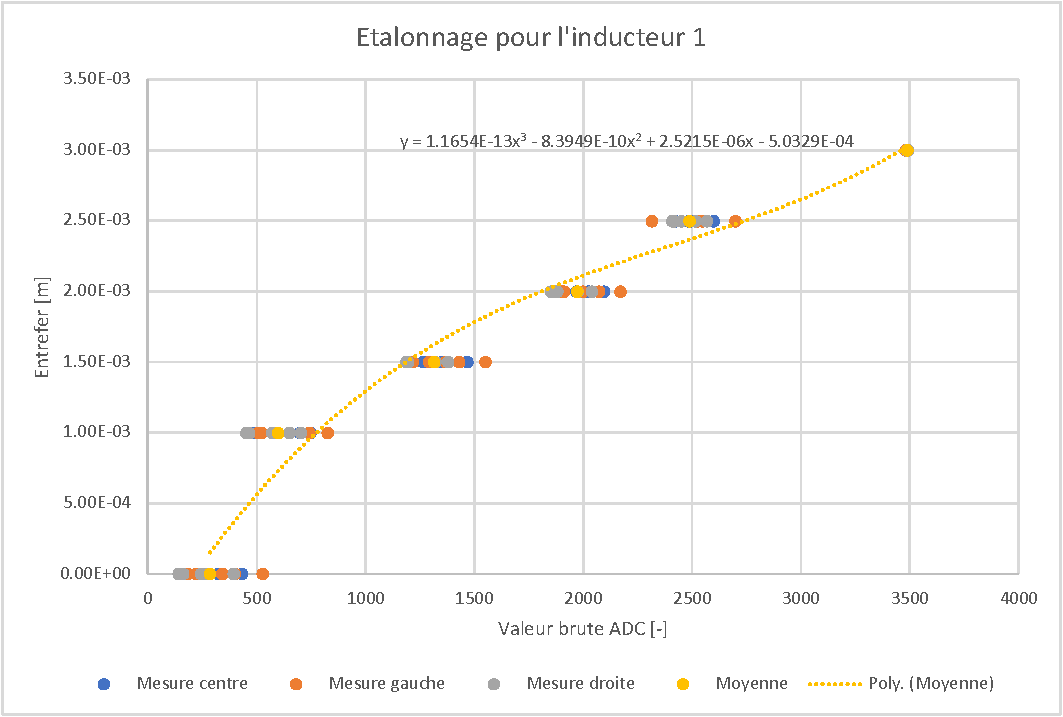
\includegraphics[width=1\linewidth]{assets/Chap3/EtaADCPol3/EtaADCPol3-1.pdf}
    \caption{Graphique d'étalonnage de l'ADC de l'inducteur 1 (polynome d'ordre 3)}
    \label{fig:Ind1Pol3}
\end{figure}

\begin{figure}[H]
    \centering
    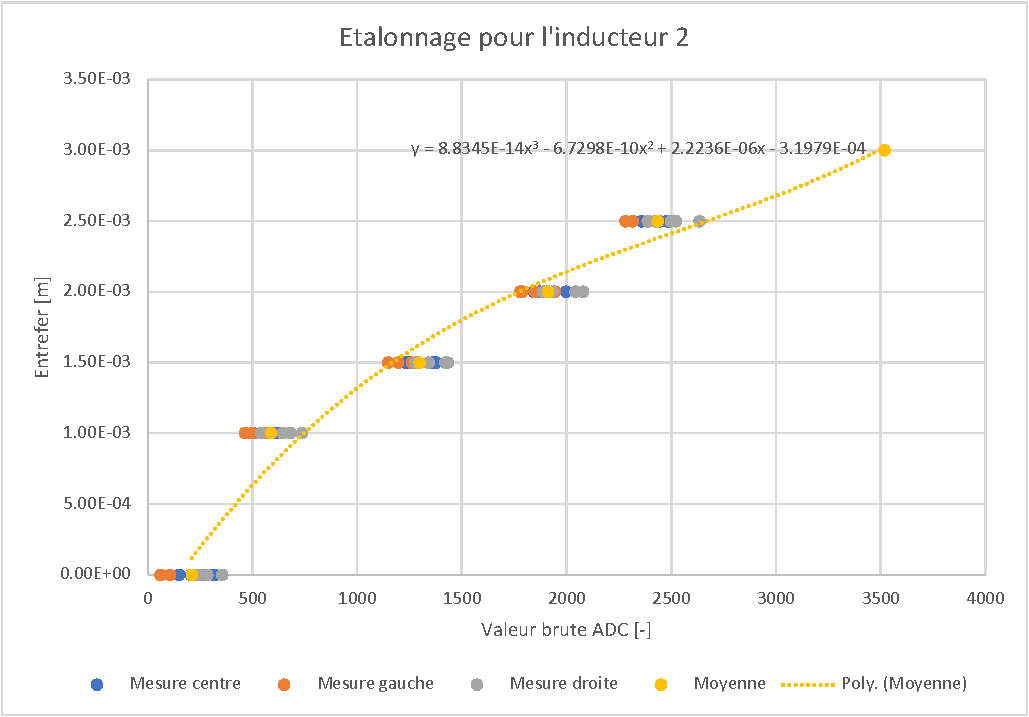
\includegraphics[width=1\linewidth]{assets/Chap3/EtaADCPol3/EtaADCPol3-2.pdf}
    \caption{Graphique d'étalonnage de l'ADC de l'inducteur 2 (polynome d'ordre 3)}
    \label{fig:Ind2Pol3}
\end{figure}

\begin{figure}[H]
    \centering
    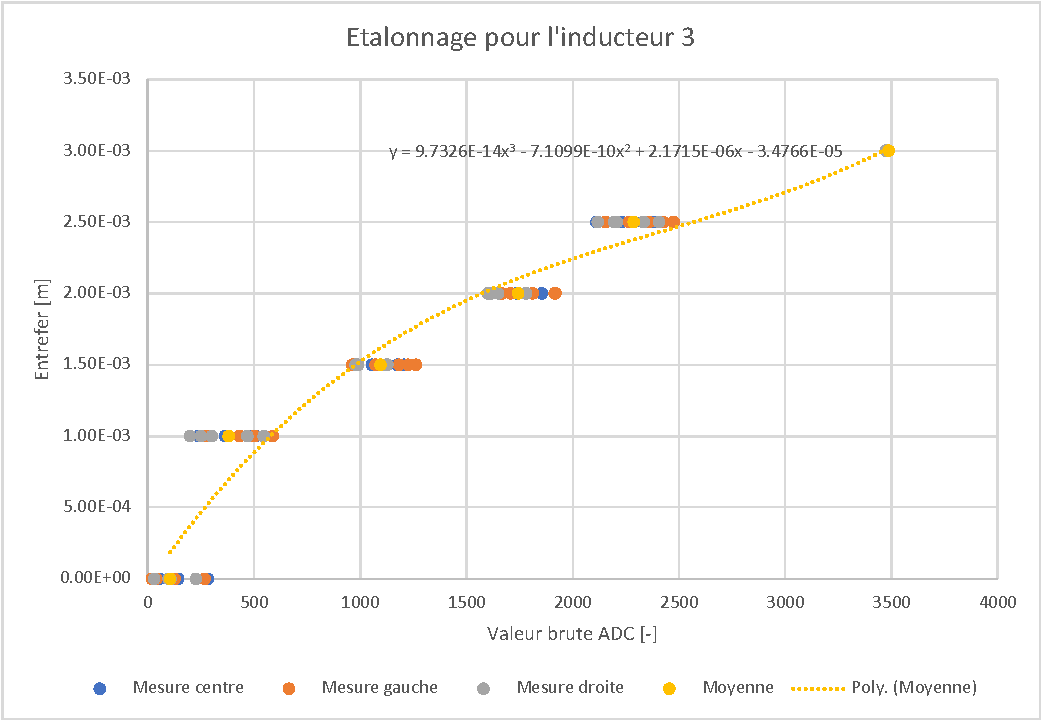
\includegraphics[width=1\linewidth]{assets/Chap3/EtaADCPol3/EtaADCPol3-3.pdf}
    \caption{Graphique d'étalonnage de l'ADC de l'inducteur 3 (polynome d'ordre 3)}
    \label{fig:Ind3Pol3}
\end{figure}

\begin{figure}[H]
    \centering
    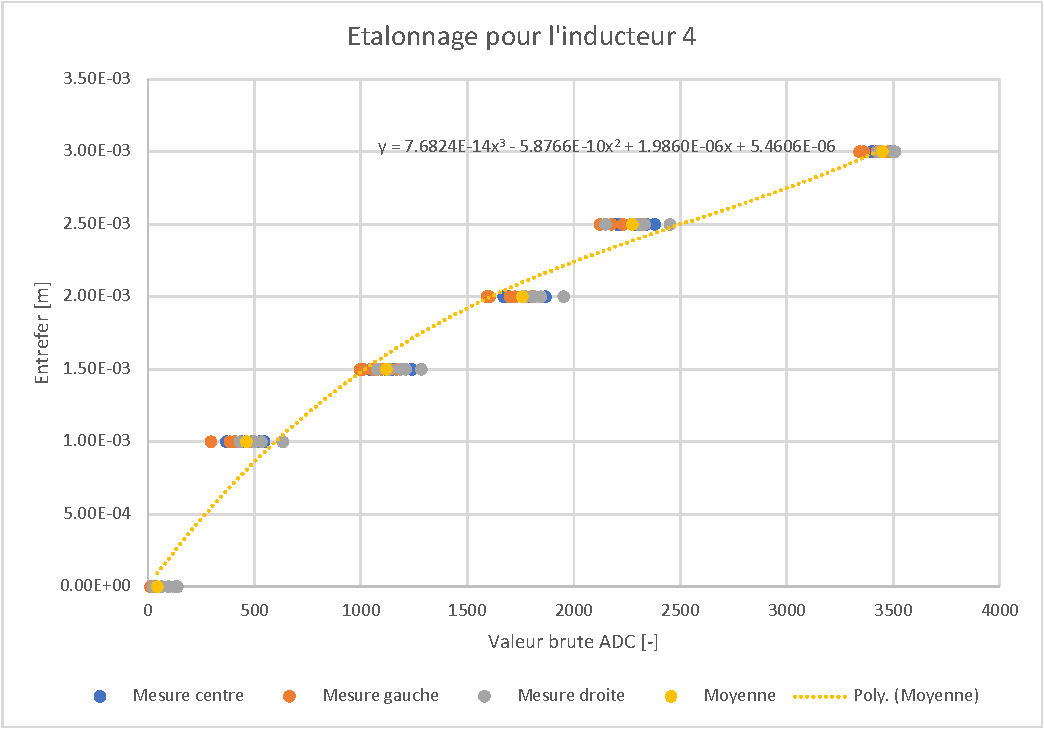
\includegraphics[width=1\linewidth]{assets/Chap3/EtaADCPol3/EtaADCPol3-4.pdf}
    \caption{Graphique d'étalonnage de l'ADC de l'inducteur 4 (polynome d'ordre 3)}
    \label{fig:Ind4Pol3}
\end{figure}

Les performances n'étant toujours pas satisfaisantes, un dernier essai reposant sur une simple équation linéaire a été mené, donnant les tracés des figures \ref{fig:Ind1Lin}, \ref{fig:Ind2Lin}, \ref{fig:Ind3Lin} et \ref{fig:Ind4Lin} :

\begin{figure}[H]
    \centering
    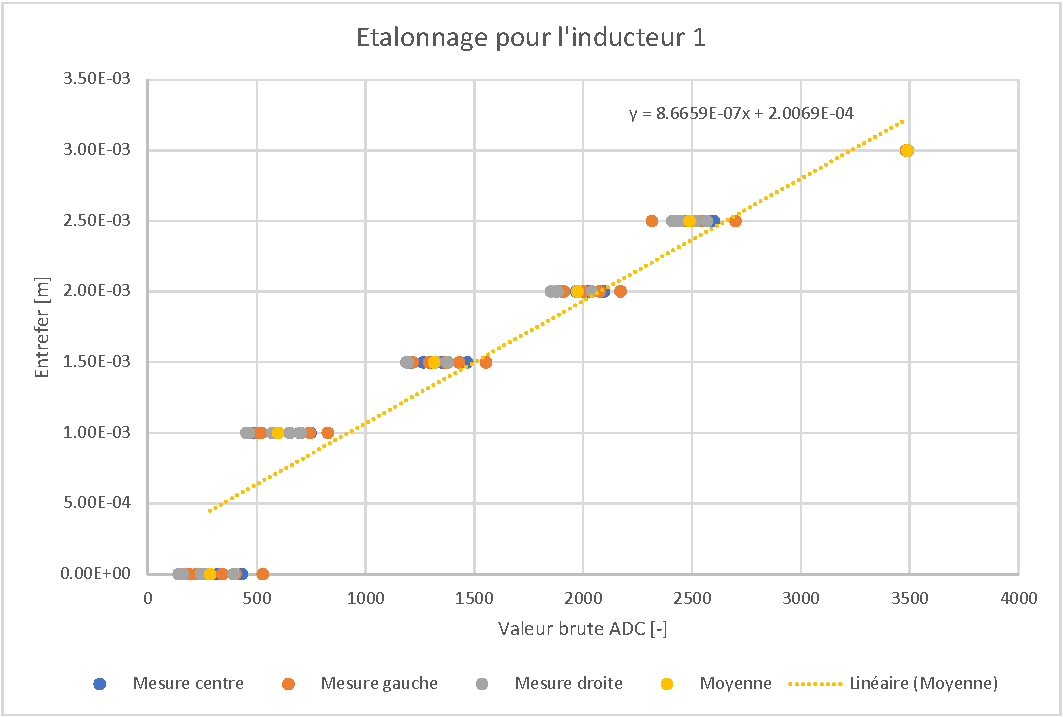
\includegraphics[width=1\linewidth]{assets/Chap3/EtaADCLin/EtaADCLin-1.pdf}
    \caption{Graphique d'étalonnage de l'ADC de l'inducteur 1 (courbe linéaire)}
    \label{fig:Ind1Lin}
\end{figure}

\begin{figure}[H]
    \centering
    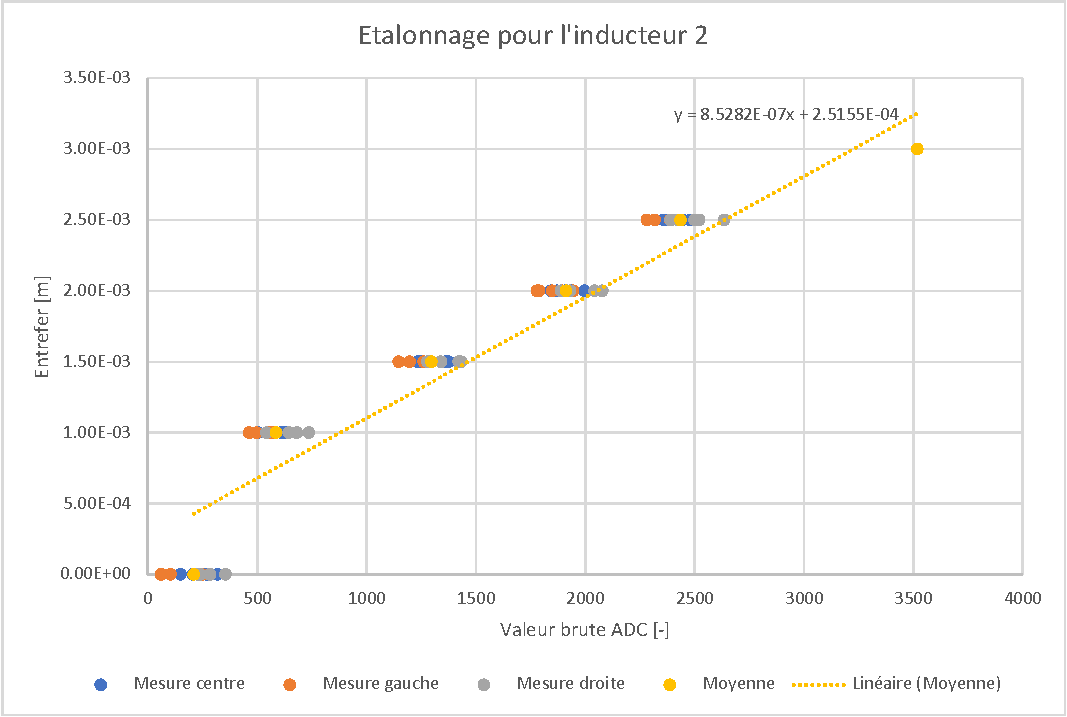
\includegraphics[width=1\linewidth]{assets/Chap3/EtaADCLin/EtaADCLin-2.pdf}
    \caption{Graphique d'étalonnage de l'ADC de l'inducteur 2 (courbe linéaire)}
    \label{fig:Ind2Lin}
\end{figure}

\begin{figure}[H]
    \centering
    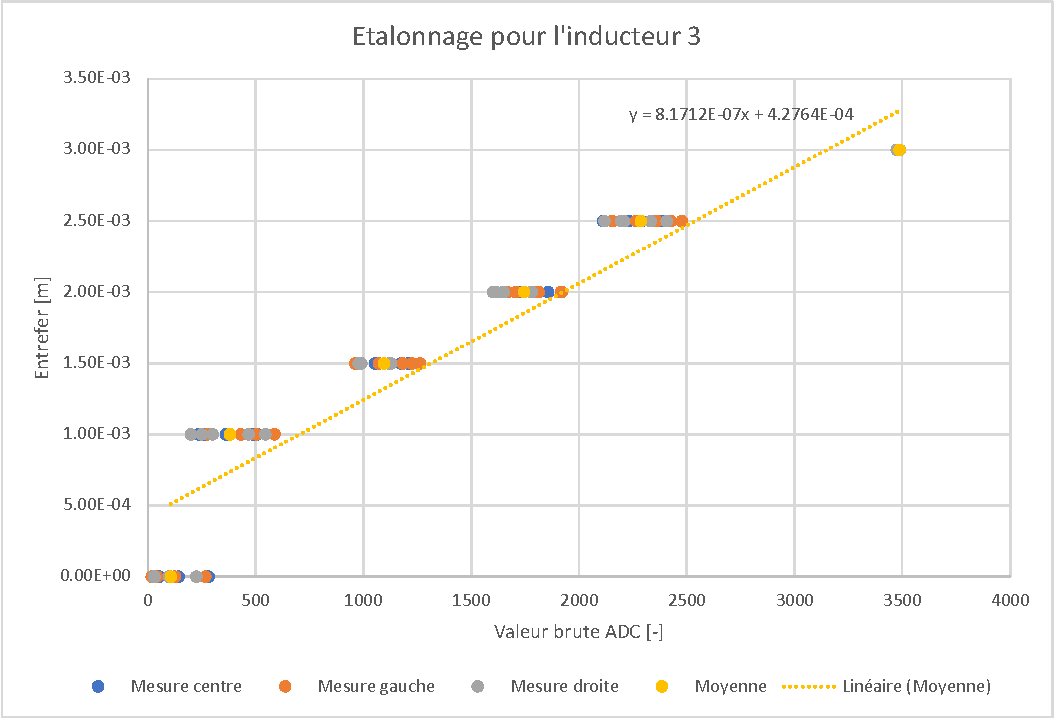
\includegraphics[width=1\linewidth]{assets/Chap3/EtaADCLin/EtaADCLin-3.pdf}
    \caption{Graphique d'étalonnage de l'ADC de l'inducteur 3 (courbe linéaire)}
    \label{fig:Ind3Lin}
\end{figure}

\begin{figure}[H]
    \centering
    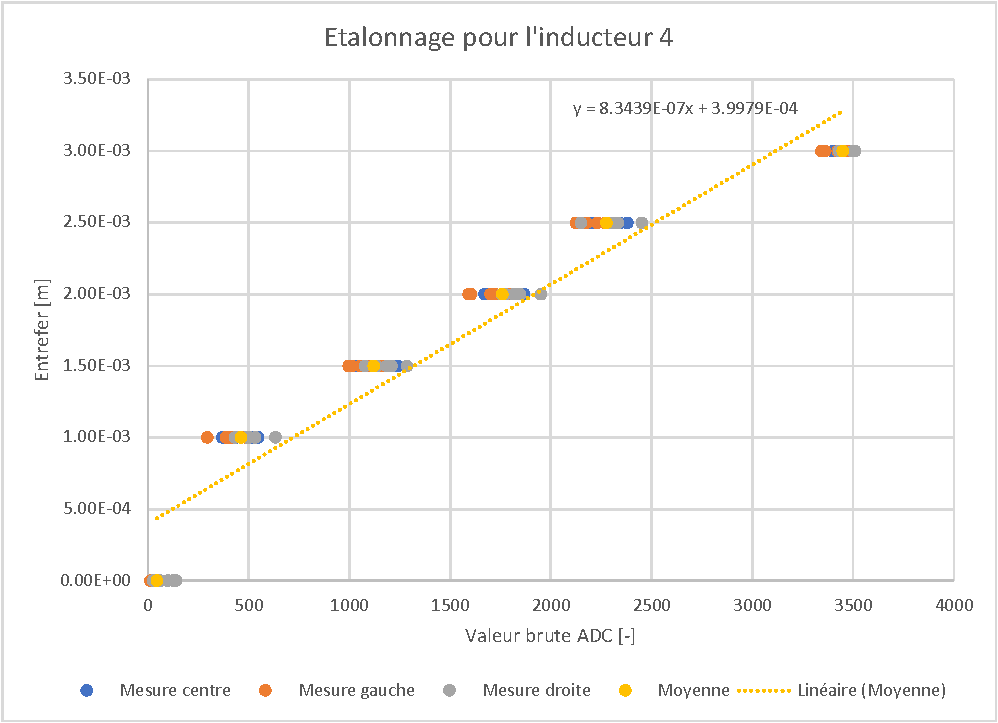
\includegraphics[width=1\linewidth]{assets/Chap3/EtaADCLin/EtaADCLin-4.pdf}
    \caption{Graphique d'étalonnage de l'ADC de l'inducteur 4 (courbe linéaire)}
    \label{fig:Ind4Lin}
\end{figure}

\subsection{Analyse des résultats}
Le traitement des signaux issus des capteurs de position n'a pas été concluant. Les diverses corrections appliquées présentaient régulièrement de faibles erreurs relatives d'un point de vue théorique, mais ne permettaient jamais d'atteindre un résultat satisfaisant en pratique.

La dernière correction linéaire testée n'a également apporté aucune amélioration.

Un phénomène récurrent lors de l'application de ces corrections était le contact brusque des inducteurs contre le rail, le système se stabilisant dans cet état de butée. Ce comportement pointe davantage vers une instabilité liée à la boucle de régulation plutôt qu'à un défaut exclusif de calibration des capteurs de position.

Il est toutefois intéressant de noter que la calibration « Teach-In » de l'ensemble des capteurs à un niveau de référence commun a semblé améliorer légèrement la stabilité de maintien de la maquette.

\section{Conclusion des mesures}
Les premières mesures effectuées sur l'ensemble des régulateurs ont donné d'excellents résultats, validant ainsi leur bon fonctionnement global.\\

Les relevés liés aux capteurs de courant et à leurs circuits de conditionnement ont montré des écarts par rapport aux valeurs théoriques calculées. Bien que les valeurs obtenues par la méthode inverse, telle qu'implémentée dans le code, diffèrent légèrement des prédictions, la mesure réelle du courant traversant l'inducteur et celle perçue par le capteur restent très proches. Il est donc possible de conclure que le capteur de courant fonctionne correctement.\\

Concernant les mesures de position, bien qu'elles aient régulièrement fourni des données cohérentes, aucune méthode de correction n'a permis d'optimiser efficacement la régulation. La seule intervention ayant montré un effet bénéfique sur la lévitation a été la calibration par la méthode d'apprentissage (« Teach-In ») des capteurs en fixant mécaniquement les inducteurs à un niveau identique.\\

En conclusion, l'électronique de la maquette est validée et certifiée fonctionnelle.